%! Unidad 2 — Disoluciones (teoría, ejemplos resueltos, ejercicios por apartados y prácticas)
%! Fuente: Fuentes/Quimica/Unidad 2 (capturas 489-501 y solucionario). Texto reescrito; datos de los ejercicios cambiados y recalculados.
%! Masas atómicas usadas: H 1; C 12; N 14; O 16; Na 23; S 32; Cl 35,5; K 39; Ca 40; Fe 55,8; Cu 63,5; Pb 207,2.
%! En las propiedades coligativas numéricas se usan solutos moleculares (no iónicos); el factor de van't Hoff solo aparece en un recuadro.

\section*{Para empezar: vivimos rodeados de disoluciones}
\addcontentsline{toc}{section}{Para empezar: vivimos rodeados de disoluciones}

Mira las etiquetas de los productos de tu casa: el refresco, el suavizante, el colirio, el insecticida o el kétchup indican su
\textbf{composición}, y muchas veces con números: «0,5 mg de azelastina por mL», «menos del 5\,\% de tensioactivos»,
«leche desnatada (10\,\%)». Casi todos son \textbf{mezclas}, y la mayoría, \textbf{disoluciones}: el aire que respiramos, el
agua del grifo, el suero de un hospital, el vinagre o la sangre. Además, se calcula que alrededor del 90\,\% de las reacciones
químicas ocurren en disolución, y casi todas ellas en agua.

En esta unidad aprenderemos a distinguir los tipos de mezclas, a expresar cuánto soluto hay en una disolución, a prepararlas en
el laboratorio y a explicar por qué el agua con sal hierve a más temperatura, por qué se echa sal en las carreteras heladas o por
qué no se puede beber agua de mar.

%========================================================================================
\section{Recuerda de la ESO}\label{sec:ud2-eso}
%========================================================================================

\paragraph{Mezclas homogéneas y heterogéneas.} Una \textbf{mezcla} está formada por dos o más sustancias puras que se pueden
separar por métodos físicos. Si presenta una sola fase y todas sus porciones tienen la misma composición y propiedades, es una
\textbf{mezcla homogénea}; sus componentes se separan por destilación, cristalización o cromatografía. Si a simple vista se
distingue más de una fase, es una \textbf{mezcla heterogénea}, y se separa por filtración, decantación o separación magnética.

\paragraph{Propiedades físicas y químicas.} Las \textbf{propiedades físicas} se miden sin que la sustancia cambie (masa,
volumen, densidad, puntos de fusión y ebullición). Las \textbf{propiedades químicas} se ponen de manifiesto cuando la sustancia
reacciona y se transforma en otra (el calor de combustión o la reactividad).

\paragraph{Sustancias polares y apolares.} Los átomos de los no metales se unen \textbf{compartiendo electrones} (enlace
covalente) y forman \textbf{moléculas}, que son neutras. Si la carga se reparte por igual, la molécula es \textbf{apolar}
(\ch{O2}, \ch{Cl2}, \ch{CO2}, \ch{CCl4}); si se acumula más carga negativa en una zona y positiva en otra, es \textbf{polar}
(\ch{H2O}, \ch{HCl}, \ch{NH3}, \ch{CO}). En el caso extremo, las cargas se separan del todo y se forman iones: es el
\textbf{enlace iónico} (\ch{NaCl}).

\paragraph{Evaporación y ebullición.} Las dos son formas de vaporización. La \textbf{ebullición} se produce en toda la masa del
líquido a una temperatura fija (que depende de la presión); la \textbf{evaporación} ocurre a cualquier temperatura, pero solo en
la superficie libre del líquido.

\begin{exercise}
    Indica el estado de agregación, a temperatura ambiente, de estas sustancias y si están formadas por moléculas polares,
    apolares o por otro tipo de partículas: a) etanol; b) metano, \ch{CH4}; c) cloruro de hidrógeno; d) hierro.
    \begin{solu}
        a) \textcolor{red}{Líquido, polar} (tiene un grupo \ch{-OH}). b) \textcolor{red}{Gas, apolar} (molécula simétrica).
        c) \textcolor{red}{Gas, polar} (el cloro atrae más los electrones). d) \textcolor{red}{Sólido; no está formado por moléculas},
        sino por átomos unidos por enlace metálico.
    \end{solu}
\end{exercise}

%========================================================================================
\section{Tipos de mezclas}\label{sec:ud2-mezclas}
%========================================================================================

En una mezcla suele distinguirse una \textbf{fase dispersante}, el medio continuo, y una \textbf{fase dispersa}, el componente
que está repartido en ella, normalmente en menor proporción. Según el \textbf{tamaño de las partículas de la fase dispersa}, las
mezclas se clasifican en tres grupos (figura~\ref{fig:ud2-tipos}).

\begin{itemize}
    \item \textbf{Mezclas heterogéneas.} Las partículas miden más de \qty{1000}{\nm} (\qty{e-6}{\m}): se ven a simple vista o al
    microscopio óptico. Cada componente conserva sus propiedades y el aspecto cambia de una zona a otra. Un caso importante son
    las \textbf{suspensiones}: un sólido fino repartido en un líquido, inestable y de aspecto turbio, que acaba sedimentando (por
    eso algunos jarabes indican «agítese antes de usar»).
    \item \textbf{Coloides o sistemas coloidales.} Las partículas, llamadas \textbf{micelas}, miden entre 1 y \qty{1000}{\nm}.
    Parecen homogéneos (a veces lechosos o nebulosos), no sedimentan en reposo y no se separan por filtración, pero
    \textbf{dispersan la luz}: un haz de luz se ve al atravesarlos (\textbf{efecto Tyndall}), como los rayos de sol en la niebla.
    Además, sus micelas tienen movimiento browniano, pueden estar cargadas y adsorben otras sustancias en su superficie, lo que les
    da mucho interés industrial (alimentación, pinturas, cosmética).
    \item \textbf{Disoluciones.} Las partículas son del orden de \qty{1}{\nm} o menores (moléculas o iones): no se ven ni al
    microscopio, no sedimentan, no se separan por filtración y el haz de luz no se ve al atravesarlas. Son transparentes (salvo las
    sólidas), tienen la misma composición en todos sus puntos y, a diferencia de las sustancias puras, sus propiedades (densidad,
    punto de ebullición…) dependen de la composición.
\end{itemize}

\begin{figure}[H]
    \centering
    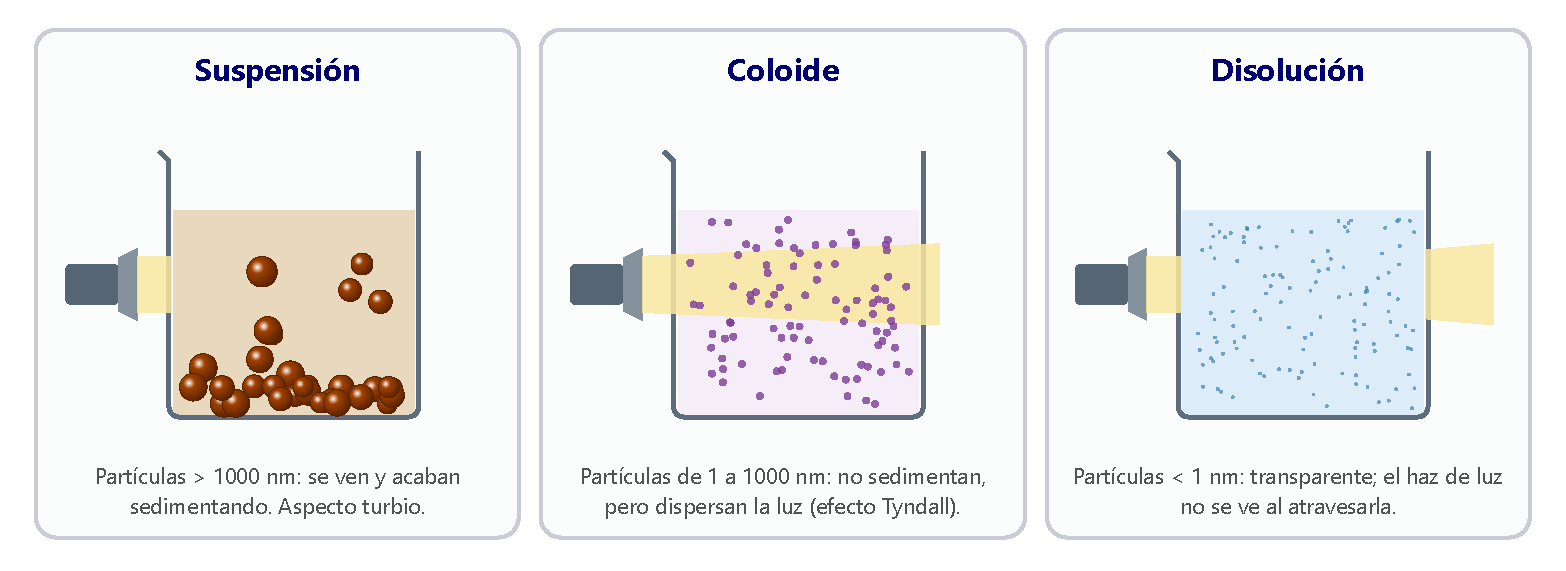
\includegraphics[width=0.95\textwidth]{images/UD2/tipos_mezclas}
    \caption{Un haz de luz permite distinguir un coloide de una disolución (efecto Tyndall).}
    \label{fig:ud2-tipos}
\end{figure}

Los coloides reciben nombres distintos según el estado de la fase dispersante y de la fase dispersa:

\begin{table}[H]
    \centering
    \caption{Tipos de coloides}
    \vspace{-5pt}
    \begin{tabular}{@{}lccc@{}}
        \toprule
        & \multicolumn{3}{c}{\textbf{Fase dispersa}} \\
        \cmidrule(l){2-4}
        \makecell{\textbf{Fase} \\ \textbf{dispersante}} & \textbf{Gas} & \textbf{Líquido} & \textbf{Sólido} \\
        \midrule
        Gas & \makecell{(siempre forman \\ disolución)} & \makecell{Aerosol líquido \\ (niebla, nubes)} & \makecell{Aerosol sólido \\ (humo, polvo)} \\[3pt]
        Líquido & \makecell{Espuma \\ (nata montada)} & \makecell{Emulsión \\ (leche, mayonesa)} & \makecell{Sol \\ (pinturas, tinta china)} \\[3pt]
        Sólido & \makecell{Espuma sólida \\ (piedra pómez)} & \makecell{Gel \\ (gelatina, queso)} & \makecell{Sol sólido \\ (vidrio de color)} \\
        \bottomrule
    \end{tabular}
    \label{tab:ud2-coloides}
\end{table}

\begin{exercise}
    Clasifica como mezcla heterogénea (suspensión), coloide o disolución: a) agua del grifo; b) niebla; c) zumo de naranja con
    pulpa; d) mayonesa; e) acero; f) arena con agua; g) gelatina; h) aire limpio.
    \begin{solu}
        \textcolor{red}{Disoluciones: a, e, h. Coloides: b (aerosol líquido), d (emulsión), g (gel). Heterogéneas: c y f
        (suspensiones).}
    \end{solu}
\end{exercise}

\begin{exercise}
    ¿Cómo distinguirías, con una linterna, un vaso de agua con un poco de leche de un vaso de agua con azúcar?
    \begin{solu}
        \textcolor{red}{Por el efecto Tyndall}: en el agua con leche (coloide) se ve el haz de luz al atravesarla; en el agua con
        azúcar (disolución) el haz no se ve.
    \end{solu}
\end{exercise}

%========================================================================================
\section{Características de las disoluciones}\label{sec:ud2-caracteristicas}
%========================================================================================

Una \textbf{disolución} es una mezcla homogénea: cualquier porción tiene la misma composición y las mismas propiedades. Sus
componentes son:

\begin{itemize}
    \item \textbf{Disolvente}: la fase dispersante. Suele ser el componente mayoritario y tiene el mismo estado de agregación que
    la disolución. Las \textbf{disoluciones acuosas}, en las que el disolvente es agua, son las más importantes: el agua disuelve
    tantas sustancias que se le llama \emph{disolvente universal}.
    \item \textbf{Soluto}: la fase dispersa, normalmente en menor proporción. Puede haber varios, y sus partículas disueltas pueden
    ser moléculas o iones.
\end{itemize}

\begin{table}[H]
    \centering
    \caption{Disoluciones según el estado de sus componentes}
    \vspace{-5pt}
    \begin{tabular}{@{}cccl@{}}
        \toprule
        \textbf{Disolvente} & \textbf{Soluto} & \textbf{Disolución} & \textbf{Ejemplo} \\
        \midrule
        Gas & Gas & Gas & Aire \\[3pt]
        Líquido & Gas & Líquido & Refresco con gas (\ch{CO2} en agua) \\[3pt]
        Líquido & Líquido & Líquido & Alcohol sanitario (etanol y agua) \\[3pt]
        Líquido & Sólido & Líquido & Agua de mar \\[3pt]
        Sólido & Gas & Sólido & Hidrógeno en paladio \\[3pt]
        Sólido & Líquido & Sólido & Amalgama de mercurio en plata \\[3pt]
        Sólido & Sólido & Sólido & Bronce (cobre y estaño) \\
        \bottomrule
    \end{tabular}
    \label{tab:ud2-tipos-disoluciones}
\end{table}

\subsection{El proceso de disolución}

Para que se forme una disolución, las partículas de soluto tienen que repartirse de manera uniforme entre las de disolvente. Esto
ocurre en tres pasos:
\begin{enumerate}
    \item Las partículas de soluto se separan entre sí, venciendo las fuerzas \textbf{soluto-soluto}.
    \item Las partículas de disolvente se separan, venciendo las fuerzas \textbf{disolvente-disolvente}.
    \item Las partículas de soluto y de disolvente se atraen (fuerzas \textbf{soluto-disolvente}). Cada partícula de soluto queda
    rodeada de moléculas de disolvente: es la \textbf{solvatación}, o \textbf{hidratación} si el disolvente es agua
    (figura~\ref{fig:ud2-nacl}).
\end{enumerate}

\begin{figure}[H]
    \centering
    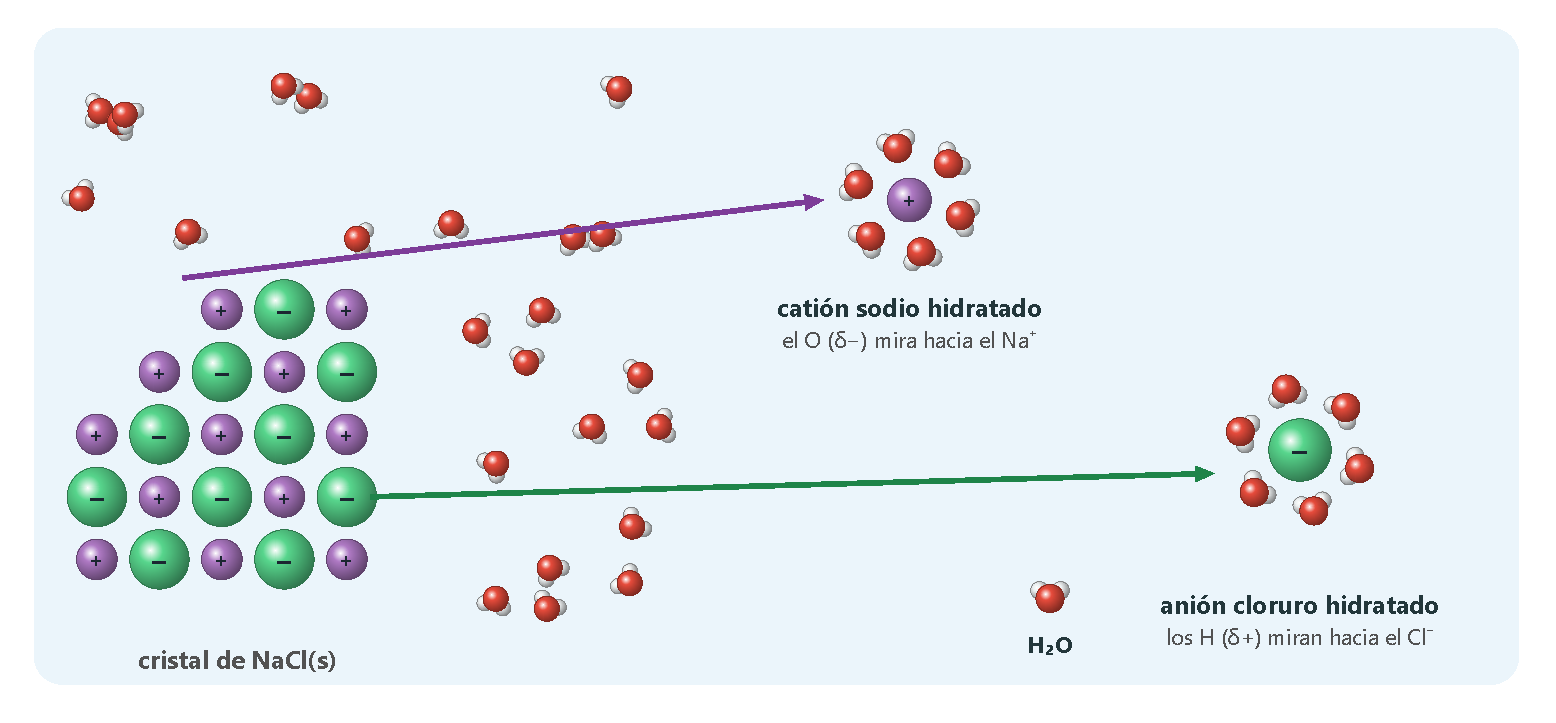
\includegraphics[width=0.9\textwidth]{images/UD2/disolucion_nacl}
    \caption{Disolución del cloruro de sodio: las moléculas de agua, polares, arrancan los iones del cristal y los rodean.}
    \label{fig:ud2-nacl}
\end{figure}

La sustancia se disuelve si las fuerzas soluto-disolvente son \textbf{más intensas} que las que hay que romper. Por eso, en
general, \textbf{«semejante disuelve a semejante»}: los solutos polares e iónicos se disuelven bien en disolventes polares (la sal
o el azúcar en agua), y los apolares, en disolventes apolares (el aceite no se disuelve en agua, pero sí en gasolina).

\paragraph{Factores que favorecen la disolución.} Todo lo que aumente el contacto entre soluto y disolvente acelera la
disolución de un sólido: que esté en \textbf{polvo} (más superficie de contacto), \textbf{agitar} (acerca disolvente nuevo a la
superficie del soluto) y \textbf{calentar} (las partículas se mueven más deprisa y se separan con más facilidad).

\begin{exercise}
    Explica por qué: a) el aceite no se disuelve en agua y sí en gasolina; b) un terrón de azúcar tarda más en disolverse que una
    cucharada de azúcar glas; c) el yodo, \ch{I2}, se disuelve mejor en tetracloruro de carbono que en agua.
    \begin{solu}
        a) \textcolor{red}{El aceite es apolar}: las fuerzas entre sus moléculas y las del agua (polar) son débiles; con la
        gasolina (apolar) sí son comparables. b) \textcolor{red}{El azúcar glas tiene mucha más superficie de contacto}. c)
        \textcolor{red}{El \ch{I2} y el \ch{CCl4} son apolares}: «semejante disuelve a semejante».
    \end{solu}
\end{exercise}

%========================================================================================
\section{Concentración de una disolución}\label{sec:ud2-concentracion}
%========================================================================================

La \textbf{concentración} relaciona la \textbf{cantidad de soluto} con la cantidad de disolución (o de disolvente). Es una
\textbf{propiedad intensiva}: no depende del tamaño de la muestra; un vaso y una cucharada de la misma disolución tienen la misma
concentración. Puede expresarse:

\begin{itemize}
    \item \textbf{Cualitativamente}: una disolución es \textbf{diluida} si tiene poco soluto, \textbf{concentrada} si tiene mucho y
    \textbf{saturada} si tiene el máximo posible.
    \item \textbf{Cuantitativamente}: con un número y su unidad. Las unidades se clasifican en \textbf{físicas}, que no tienen en
    cuenta la naturaleza del soluto, y \textbf{químicas}, que sí lo hacen (usan la cantidad de sustancia).
\end{itemize}

\subsection{Unidades físicas de concentración}

\begin{definition}[Porcentaje en masa]
    Gramos de soluto que hay en \qty{100}{\gram} de disolución:
    \[ \%\ \text{en masa} = \frac{m_{\text{soluto}}}{m_{\text{disolución}}} \cdot 100 \qquad (m_{\text{disolución}} = m_{\text{soluto}} + m_{\text{disolvente}}) \]
\end{definition}

\begin{definition}[Porcentaje en volumen]
    Volumen de soluto que hay en 100 unidades de volumen de disolución:
    \[ \%\ \text{en volumen} = \frac{V_{\text{soluto}}}{V_{\text{disolución}}} \cdot 100 \]
    En las bebidas alcohólicas se expresa en \textbf{grados}: \(1^{\circ}\) equivale al 1\,\% en volumen.
\end{definition}

\begin{definition}[Concentración en masa]
    Masa de soluto por unidad de volumen de disolución. Suele darse en \unit{\gram\per\litre} (en el SI, \unit{\kilo\gram\per\cubic\metre}):
    \[ \gamma = \frac{m_{\text{soluto}}}{V_{\text{disolución}}} \]
\end{definition}

\begin{remark}
    \textbf{¡Los volúmenes no son aditivos!} La masa de una disolución es siempre la suma de las masas de sus componentes, pero su
    volumen no: al mezclarse, las partículas se reacomodan y el volumen suele ser algo menor que la suma. Al mezclar \qty{50}{\mL}
    de etanol con \qty{50}{\mL} de agua se obtienen unos \qty{97}{\mL}. Por eso, salvo que el enunciado diga lo contrario, no se
    suman volúmenes.
\end{remark}

\paragraph{Concentración en masa y densidad.} Las dos se expresan, por ejemplo, en \unit{\gram\per\litre}, pero
\textbf{no miden lo mismo}:
\[ \gamma = \frac{m_{\text{soluto}}}{V_{\text{disolución}}} \qquad\qquad d = \frac{m_{\text{disolución}}}{V_{\text{disolución}}} = \frac{m_{\text{soluto}} + m_{\text{disolvente}}}{V_{\text{disolución}}} \]
La densidad de una sustancia pura es una propiedad característica; la de una disolución, no, porque depende de su concentración
(un huevo flota en agua muy salada y se hunde en agua dulce). La densidad sirve para pasar de masa de disolución a volumen de
disolución.

\paragraph{Partes por millón.} Para concentraciones muy pequeñas se usan las \textbf{partes por millón} (\unit{\ppm}): unidades
de soluto por cada millón de unidades de disolución, en masa o en volumen. En disoluciones acuosas diluidas,
\(\qty{1}{\ppm} \approx \qty{1}{\milli\gram\per\litre}\). Por ejemplo, más de \qty{50}{\ppm} en volumen de monóxido de carbono
en el aire es peligroso para la salud.

\begin{example}
    \textbf{Chocolate y vino.} a) Una tableta de \qty{200}{\gram} indica «70\,\% de cacao». ¿Cuánto cacao contiene?
    b) ¿Cuánto etanol hay en una botella de \qty{750}{\mL} de vino de \ang{13}?

    \textbf{Solución.} a) \(m_{\text{cacao}} = \qty{200}{\gram} \cdot \dfrac{\qty{70}{\gram}\ \text{cacao}}{\qty{100}{\gram}\ \text{tableta}} = \qty{140}{\gram}\) de cacao.

    b) \ang{13} significa 13\,\% en volumen: \(V_{\text{etanol}} = \qty{750}{\mL} \cdot \dfrac{13}{100} = \qty{97.5}{\mL}\) de etanol.
\end{example}

\begin{example}
    \textbf{Concentración en masa.} Se disuelven \qty{30}{\gram} de hidróxido de sodio en agua hasta tener \qty{250}{\mL} de
    disolución. Calcula su concentración en \unit{\gram\per\litre}.

    \textbf{Solución.} \(\gamma = \dfrac{\qty{30}{\gram}}{\qty{250}{\mL}} \cdot \dfrac{\qty{1000}{\mL}}{\qty{1}{\litre}} =
    \qty{120}{\gram\per\litre}\): cada litro de disolución contiene \qty{120}{\gram} de \ch{NaOH}.
\end{example}

\begin{exercise}
    Calcula el porcentaje en masa de una disolución preparada disolviendo \qty{12}{\gram} de cloruro de hidrógeno en
    \qty{140}{\gram} de agua.
    \begin{solu}
        \(\% = \dfrac{12}{12 + 140} \cdot 100 = \textcolor{red}{\qty{7.9}{\percent}}\).
    \end{solu}
\end{exercise}

\begin{exercise}
    Se mezclan \qty{250}{\gram} de sulfato de cobre(II) con \qty{1}{\litre} de agua (\(d = \qty{1}{\gram\per\mL}\)). ¿Cuál es el
    porcentaje en masa de la disolución?
    \begin{solu}
        \(m_{\text{agua}} = \qty{1000}{\gram}\): \(\% = \dfrac{250}{1250} \cdot 100 = \textcolor{red}{\qty{20}{\percent}}\).
    \end{solu}
\end{exercise}

\begin{exercise}
    Tenemos una disolución de ácido clorhídrico al 36\,\% en masa. a) ¿Qué masa de \ch{HCl} hay en \qty{400}{\gram} de disolución?
    b) ¿Qué masa de disolución contiene \qty{90}{\gram} de \ch{HCl}?
    \begin{solu}
        a) \(400 \cdot \dfrac{36}{100} = \textcolor{red}{\qty{144}{\gram}}\). b) \(90 \cdot \dfrac{100}{36} = \textcolor{red}{\qty{250}{\gram}}\) de disolución.
    \end{solu}
\end{exercise}

\begin{exercise}
    Se prepara una disolución de éter en cloroformo mezclando \qty{30}{\mL} de éter con \qty{150}{\mL} de cloroformo. Suponiendo
    los volúmenes aditivos, ¿cuál es su porcentaje en volumen?
    \begin{solu}
        \(\% = \dfrac{30}{30 + 150} \cdot 100 = \textcolor{red}{\qty{16.7}{\percent}}\) en volumen.
    \end{solu}
\end{exercise}

\begin{exercise}
    a) Calcula la concentración en \unit{\gram\per\litre} de una disolución con \qty{255}{\gram} de sulfato de cobre(II) en
    \qty{3}{\litre} de disolución. b) ¿Cuántos gramos de ácido nítrico hacen falta para preparar \qty{2.5}{\litre} de disolución
    de \qty{0.8}{\gram\per\litre}?
    \begin{solu}
        a) \(\gamma = 255/3 = \textcolor{red}{\qty{85}{\gram\per\litre}}\). b) \(m = \num{0.8} \cdot \num{2.5} = \textcolor{red}{\qty{2}{\gram}}\).
    \end{solu}
\end{exercise}

\begin{exercise}
    Una disolución acuosa de cloruro de sodio tiene una densidad de \qty{1.2}{\gram\per\cubic\cm} y una concentración de
    \qty{240}{\gram\per\litre}. a) ¿Cuál es la masa de \qty{150}{\mL} de disolución? b) ¿Cuánto \ch{NaCl} hay en
    \qty{250}{\mL}?
    \begin{solu}
        a) Con la densidad: \(m = \num{1.2} \cdot 150 = \textcolor{red}{\qty{180}{\gram}}\). b) Con la concentración:
        \(m = 240 \cdot \num{0.250} = \textcolor{red}{\qty{60}{\gram}}\) de \ch{NaCl}.
    \end{solu}
\end{exercise}

\begin{exercise}
    \label{ej:ud2-etanol}
    Se mezclan \qty{40}{\mL} de etanol (\(d = \qty{0.79}{\gram\per\mL}\)) con \qty{960}{\mL} de agua
    (\(d = \qty{1}{\gram\per\mL}\)) y se obtienen \qty{985}{\mL} de disolución. Expresa su concentración en \% en volumen,
    \unit{\gram\per\litre} y \% en masa.
    \begin{solu}
        \textcolor{blue}{\(m_{\text{etanol}} = 40 \cdot \num{0.79} = \qty{31.6}{\gram}\); \(m_{\text{agua}} = \qty{960}{\gram}\).}
        \% vol \(= 40/985 \cdot 100 = \textcolor{red}{\qty{4.06}{\percent}}\);
        \(\gamma = \num{31.6}/\num{0.985} = \textcolor{red}{\qty{32.1}{\gram\per\litre}}\);
        \% masa \(= \num{31.6}/\num{991.6} \cdot 100 = \textcolor{red}{\qty{3.19}{\percent}}\).
    \end{solu}
\end{exercise}

\begin{exercise}
    Un litro de leche semidesnatada contiene \qty{48}{\gram} de lactosa y tiene una densidad de \qty{1.03}{\gram\per\cubic\cm}.
    Calcula: a) el porcentaje en masa de lactosa; b) su concentración en \unit{\gram\per\litre}; c) la lactosa que hay en un vaso
    de \qty{150}{\mL}.
    \begin{solu}
        a) \(m_{\text{leche}} = \qty{1030}{\gram}\): \(\% = 48/1030 \cdot 100 = \textcolor{red}{\qty{4.66}{\percent}}\).
        b) \(\textcolor{red}{\qty{48}{\gram\per\litre}}\). c) \(48 \cdot \num{0.150} = \textcolor{red}{\qty{7.2}{\gram}}\).
    \end{solu}
\end{exercise}

\begin{exercise}
    En \qty{300}{\mL} de una disolución de glucosa hay \qty{15}{\gram} de soluto. Su densidad es \qty{1.02}{\gram\per\cubic\cm}.
    a) Calcula su concentración en \% en masa y en \unit{\gram\per\litre}. b) Si un niño puede tomar como mucho \qty{20}{\gram}
    de glucosa, ¿qué volumen de disolución podrá tomar como máximo?
    \begin{solu}
        a) \(m_{\text{disolución}} = 300 \cdot \num{1.02} = \qty{306}{\gram}\): \(\% = 15/306 \cdot 100 = \textcolor{red}{\qty{4.9}{\percent}}\);
        \(\gamma = 15/\num{0.3} = \textcolor{red}{\qty{50}{\gram\per\litre}}\). b) \(V = 20/50 = \qty{0.4}{\litre} = \textcolor{red}{\qty{400}{\mL}}\).
    \end{solu}
\end{exercise}

\subsection{Unidades químicas de concentración}

Tienen en cuenta la naturaleza del soluto, porque utilizan su \textbf{cantidad de sustancia} (los moles), que se calcula con la
masa molar: \(n = m/M\). Solo las sustancias puras tienen masa molar; por eso hay que calcular por separado los moles de cada
componente.

\begin{definition}[Concentración molar o molaridad]
    Moles de soluto por litro de disolución. Su unidad es el \unit{\mol\per\litre}, que se abrevia \unit{\M} («molar»):
    \[ c = \frac{n_{\text{soluto}}}{V_{\text{disolución}}\ (\unit{\litre})} \]
\end{definition}

\begin{definition}[Molalidad]
    Moles de soluto por kilogramo de \textbf{disolvente}. Su unidad es el \unit{\mol\per\kilo\gram}:
    \[ m = \frac{n_{\text{soluto}}}{m_{\text{disolvente}}\ (\unit{\kilo\gram})} \]
\end{definition}

\begin{definition}[Fracción molar]
    Moles de un componente \(i\) entre los moles totales de la disolución. No tiene unidades, y la suma de las fracciones molares
    de todos los componentes vale 1:
    \[ \chi_i = \frac{n_i}{n_{\text{total}}} \qquad\qquad \chi_{\text{soluto}} + \chi_{\text{disolvente}} = 1 \]
\end{definition}

\begin{remark}
    La molalidad es la única concentración que se refiere al disolvente y no a la disolución. Como no depende del volumen, no cambia
    con la temperatura, y por eso se usa en las propiedades coligativas. ¡Cuidado con los símbolos!: \(m\) (molalidad) y
    \(M\) (masa molar) también se usan para la masa; fíjate siempre en las unidades.
\end{remark}

\begin{table}[H]
    \centering
    \caption{Resumen de las unidades de concentración}
    \vspace{-5pt}
    \begin{tabular}{@{}lcc@{}}
        \toprule
        \textbf{Unidad} & \textbf{Expresión} & \textbf{Unidad habitual} \\
        \midrule
        Porcentaje en masa & \(\dfrac{m_{\text{soluto}}}{m_{\text{disolución}}} \cdot 100\) & \% \\[9pt]
        Porcentaje en volumen & \(\dfrac{V_{\text{soluto}}}{V_{\text{disolución}}} \cdot 100\) & \% (grados) \\[9pt]
        Concentración en masa & \(\dfrac{m_{\text{soluto}}}{V_{\text{disolución}}}\) & \unit{\gram\per\litre} \\[9pt]
        Concentración molar & \(\dfrac{n_{\text{soluto}}}{V_{\text{disolución}}}\) & \unit{\mol\per\litre} (\unit{\M}) \\[9pt]
        Molalidad & \(\dfrac{n_{\text{soluto}}}{m_{\text{disolvente}}}\) & \unit{\mol\per\kilo\gram} \\[9pt]
        Fracción molar & \(\dfrac{n_i}{n_{\text{total}}}\) & sin unidades \\
        \bottomrule
    \end{tabular}
    \label{tab:ud2-unidades}
\end{table}

\begin{example}
    \textbf{Molaridad y molalidad de una disolución de glucosa.} Se disuelven \qty{45}{\gram} de glucosa, \ch{C6H12O6}, en agua
    hasta obtener \qty{2}{\litre} de disolución, de densidad \qty{1.02}{\gram\per\cubic\cm}. Calcula: a) la concentración molar;
    b) la molalidad.

    \textbf{Solución.} \(M(\ch{C6H12O6}) = 6 \cdot 12 + 12 \cdot 1 + 6 \cdot 16 = \qty{180}{\gram\per\mol}\);
    \(n = \dfrac{45}{180} = \qty{0.25}{\mol}\).

    a) \(c = \dfrac{\qty{0.25}{\mol}}{\qty{2}{\litre}} = \qty{0.125}{\mol\per\litre}\).

    b) Con la densidad hallamos la masa de disolución y, restando el soluto, la del disolvente:
    \(m_{\text{disolución}} = \qty{2000}{\mL} \cdot \qty{1.02}{\gram\per\mL} = \qty{2040}{\gram}\);
    \(m_{\text{agua}} = 2040 - 45 = \qty{1995}{\gram}\).
    \[ m = \frac{\qty{0.25}{\mol}}{\qty{1.995}{\kilo\gram}} = \qty{0.125}{\mol\per\kilo\gram} \]
    En disoluciones acuosas diluidas, molaridad y molalidad casi coinciden.
\end{example}

\begin{example}
    \textbf{Fracción molar.} a) Un recipiente contiene \qty{280}{\gram} de nitrógeno y \qty{50}{\gram} de hidrógeno. Calcula la
    fracción molar de cada gas. b) Se disuelven \qty{46}{\gram} de etanol, \ch{C2H6O}, en \qty{500}{\gram} de agua. Calcula la
    fracción molar del etanol y la molalidad.

    \textbf{Solución.} a) \(n(\ch{N2}) = 280/28 = \qty{10}{\mol}\); \(n(\ch{H2}) = 50/2 = \qty{25}{\mol}\).
    \(\chi(\ch{N2}) = \dfrac{10}{35} = \num{0.286}\); \(\chi(\ch{H2}) = \dfrac{25}{35} = \num{0.714}\). Comprobamos que suman 1.

    b) \(n_{\text{etanol}} = 46/46 = \qty{1}{\mol}\); \(n_{\text{agua}} = 500/18 = \qty{27.8}{\mol}\).
    \(\chi_{\text{etanol}} = \dfrac{1}{1 + \num{27.8}} = \num{0.035}\); \(m = \dfrac{\qty{1}{\mol}}{\qty{0.5}{\kilo\gram}} = \qty{2}{\mol\per\kilo\gram}\).
\end{example}

\begin{example}
    \label{ex:ud2-sulfurico}
    \textbf{Una botella de ácido sulfúrico.} La etiqueta de una botella de ácido sulfúrico indica: «95\,\% de riqueza en masa;
    \(d = \qty{1.83}{\gram\per\cubic\cm}\)». Calcula su concentración en \unit{\gram\per\litre}, su concentración molar y su
    molalidad.

    \textbf{Solución.} \(M(\ch{H2SO4}) = \qty{98}{\gram\per\mol}\). Encadenamos factores de conversión partiendo de la riqueza
    (\qty{95}{\gram} de ácido por cada \qty{100}{\gram} de disolución):
    \[ \gamma = \frac{\qty{95}{\gram}\ \ch{H2SO4}}{\qty{100}{\gram}\ \text{dis.}} \cdot \frac{\qty{1.83}{\gram}\ \text{dis.}}{\qty{1}{\cubic\cm}} \cdot
    \frac{\qty{1000}{\cubic\cm}}{\qty{1}{\litre}} = \qty{1738.5}{\gram\per\litre} \]
    \[ c = \frac{\qty{1738.5}{\gram}\ \ch{H2SO4}}{\qty{1}{\litre}} \cdot \frac{\qty{1}{\mol}}{\qty{98}{\gram}} = \qty{17.7}{\mol\per\litre} \]
    Para la molalidad, en \qty{100}{\gram} de disolución hay \qty{95}{\gram} de ácido y \(100 - 95 = \qty{5}{\gram}\) de agua:
    \[ m = \frac{95/98\ \unit{\mol}}{\qty{0.005}{\kilo\gram}} = \qty{194}{\mol\per\kilo\gram} \]
\end{example}

\begin{exercise}
    ¿Qué masa de cloruro de calcio, \ch{CaCl2}, hay que disolver para obtener \qty{200}{\mL} de disolución
    \qty{0.15}{\mol\per\litre}?
    \begin{solu}
        \(n = \num{0.15} \cdot \num{0.2} = \qty{0.03}{\mol}\); \(M = \qty{111}{\gram\per\mol}\): \(m = \textcolor{red}{\qty{3.33}{\gram}}\).
    \end{solu}
\end{exercise}

\begin{exercise}
    ¿Cuántos gramos de \ch{FeCl2} hay en \qty{80}{\gram} de una disolución acuosa \qty{0.2}{\mol\per\kilo\gram}?
    \begin{solu}
        \textcolor{blue}{\(M = \qty{126.8}{\gram\per\mol}\). Por cada kg de agua hay \qty{0.2}{\mol} (\qty{25.36}{\gram}) de soluto,
        es decir, \qty{1025.36}{\gram} de disolución.} \(m = 80 \cdot \dfrac{\num{25.36}}{\num{1025.36}} = \textcolor{red}{\qty{1.98}{\gram}}\).
    \end{solu}
\end{exercise}

\begin{exercise}
    ¿Qué volumen de una disolución de maltosa, \ch{C12H22O11}, \qty{4}{\mol\per\litre} contiene \qty{150}{\gram} de maltosa?
    \begin{solu}
        \(M = \qty{342}{\gram\per\mol}\); \(n = 150/342 = \qty{0.439}{\mol}\): \(V = \num{0.439}/4 = \qty{0.110}{\litre} = \textcolor{red}{\qty{110}{\mL}}\).
    \end{solu}
\end{exercise}

\begin{exercise}
    Una mezcla contiene \qty{40}{\gram} de metanol, \ch{CH3OH}, y \qty{90}{\gram} de agua. Calcula la fracción molar de cada
    componente.
    \begin{solu}
        \(n_{\text{metanol}} = 40/32 = \qty{1.25}{\mol}\); \(n_{\text{agua}} = 90/18 = \qty{5}{\mol}\):
        \(\chi_{\text{metanol}} = \textcolor{red}{\num{0.2}}\); \(\chi_{\text{agua}} = \textcolor{red}{\num{0.8}}\).
    \end{solu}
\end{exercise}

\begin{exercise}
    Calcula la concentración en \unit{\gram\per\litre}, la concentración molar y la molalidad de un ácido clorhídrico comercial
    del 35\,\% en masa y densidad \qty{1.18}{\gram\per\mL}.
    \begin{solu}
        \(\gamma = \num{0.35} \cdot 1180 = \textcolor{red}{\qty{413}{\gram\per\litre}}\); \(c = 413/\num{36.5} = \textcolor{red}{\qty{11.3}{\mol\per\litre}}\);
        \(m = \dfrac{35/\num{36.5}}{\num{0.065}} = \textcolor{red}{\qty{14.8}{\mol\per\kilo\gram}}\).
    \end{solu}
\end{exercise}

\begin{exercise}
    Repite el ejercicio anterior para un ácido nítrico comercial del 65\,\% en masa y densidad \qty{1.40}{\gram\per\mL}.
    \begin{solu}
        \(\gamma = \textcolor{red}{\qty{910}{\gram\per\litre}}\); \(c = 910/63 = \textcolor{red}{\qty{14.4}{\mol\per\litre}}\);
        \(m = \dfrac{65/63}{\num{0.035}} = \textcolor{red}{\qty{29.5}{\mol\per\kilo\gram}}\).
    \end{solu}
\end{exercise}

%========================================================================================
\section{Preparación de una disolución}\label{sec:ud2-preparacion}
%========================================================================================

Preparar disoluciones de concentración conocida es una tarea habitual en un laboratorio, pero también en una farmacia, un
hospital o una industria alimentaria. Veremos cómo preparar una disolución líquida a partir de un \textbf{soluto sólido} y a
partir de \textbf{otra disolución} más concentrada. En el laboratorio, recuerda: protege ojos y manos, usa cada instrumento como
corresponde y mide masas y volúmenes con cuidado.

\subsection{A partir de un soluto sólido}

Primero se \textbf{calcula} la masa de soluto necesaria. Después (figura~\ref{fig:ud2-prep-solido}):
\begin{enumerate}[label=\numberballgreen]
    \item Se coloca un vidrio de reloj en la balanza, se pulsa «tara» y se \textbf{pesa} el soluto con una espátula.
    \item Se \textbf{disuelve} en un vaso de precipitados con un poco de agua destilada (menos del volumen final), agitando con una
    varilla.
    \item Se \textbf{trasvasa} a un matraz aforado del volumen deseado con ayuda de un embudo. Se enjuaga el vaso con un poco de
    agua y se añade también al matraz, para no perder soluto.
    \item Se añade agua destilada hasta cerca de la marca y se termina con un cuentagotas: se \textbf{enrasa} cuando la parte
    inferior del menisco toca la marca de aforo, mirando a la altura de los ojos.
    \item Se tapa, se agita para homogeneizar y se \textbf{etiqueta} con la fórmula del soluto, la concentración y la fecha.
\end{enumerate}

\begin{figure}[H]
    \centering
    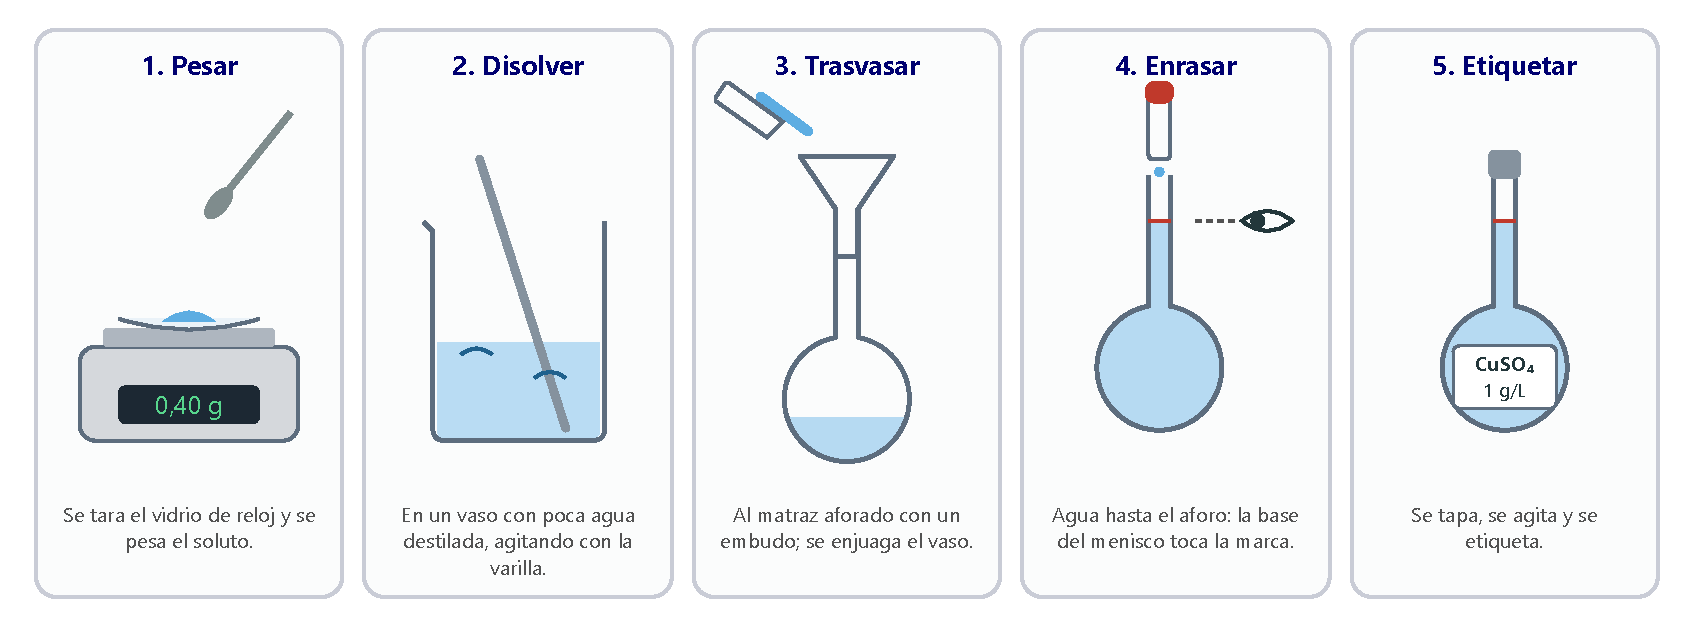
\includegraphics[width=\textwidth]{images/UD2/preparacion_solido}
    \caption{Pasos para preparar una disolución a partir de un soluto sólido.}
    \label{fig:ud2-prep-solido}
\end{figure}

\begin{example}
    \textbf{Disolución de sulfato de cobre(II).} ¿Cómo prepararías \qty{250}{\mL} de una disolución de \ch{CuSO4}
    \qty{0.1}{\mol\per\litre}?

    \textbf{Solución.} \(M(\ch{CuSO4}) = \num{63.5} + 32 + 4 \cdot 16 = \qty{159.5}{\gram\per\mol}\).
    \[ \qty{0.250}{\litre} \cdot \frac{\qty{0.1}{\mol}}{\qty{1}{\litre}} \cdot \frac{\qty{159.5}{\gram}}{\qty{1}{\mol}} = \qty{3.99}{\gram} \]
    Se pesan \qty{3.99}{\gram} de \ch{CuSO4}, se disuelven en un vaso con unos \qty{100}{\mL} de agua destilada, se pasan a un
    matraz aforado de \qty{250}{\mL} y se enrasa.
\end{example}

\subsection{A partir de otra disolución: dilución}

\textbf{Diluir} es añadir disolvente a una disolución para obtener otra de \textbf{menor} concentración. La clave es que, al
añadir disolvente, \textbf{los moles de soluto no cambian}: los que tomamos de la disolución concentrada (\(c_1\), \(V_1\)) son
los que habrá en la diluida (\(c_2\), \(V_2\)):
\[ n = c_1 V_1 = c_2 V_2 \]
Con una \textbf{pipeta} se toma el volumen \(V_1\) de la disolución concentrada, se vierte en un matraz aforado de volumen \(V_2\)
que ya contenga algo de agua destilada y se enrasa (figura~\ref{fig:ud2-dilucion}).

\begin{figure}[H]
    \centering
    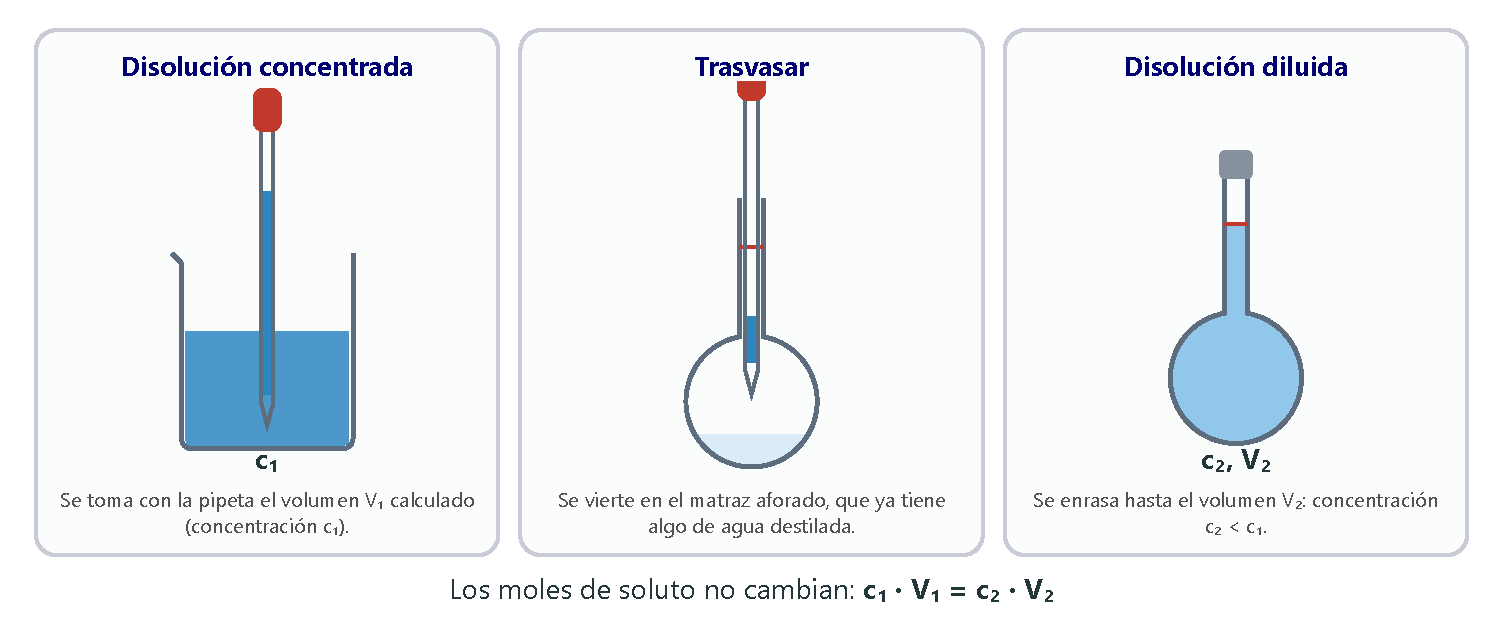
\includegraphics[width=0.85\textwidth]{images/UD2/dilucion}
    \caption{Preparación de una disolución diluida a partir de otra concentrada.}
    \label{fig:ud2-dilucion}
\end{figure}

\begin{remark}
    \textbf{Seguridad: el ácido sobre el agua.} Al diluir ácidos concentrados (sobre todo el sulfúrico) se desprende mucho calor.
    Por eso se vierte siempre \textbf{el ácido sobre el agua}, poco a poco, y nunca al revés: el agua añadida sobre el ácido podría
    hervir de golpe y salpicar.
\end{remark}

\begin{example}
    \textbf{Ácido nítrico diluido a partir del comercial.} Hay que preparar \qty{250}{\mL} de ácido nítrico
    \qty{0.4}{\mol\per\litre} a partir de un ácido comercial del 65\,\% en masa y densidad \qty{1.40}{\gram\per\mL}. ¿Qué
    volumen del comercial se necesita?

    \textbf{Solución.} 1) Moles de \ch{HNO3} necesarios: \(n = \num{0.4} \cdot \num{0.250} = \qty{0.1}{\mol}\).

    2) Volumen de ácido comercial que los contiene, encadenando masa molar, riqueza y densidad:
    \[ \qty{0.1}{\mol} \cdot \frac{\qty{63}{\gram}\ \ch{HNO3}}{\qty{1}{\mol}} \cdot \frac{\qty{100}{\gram}\ \text{dis.}}{\qty{65}{\gram}\ \ch{HNO3}} \cdot
    \frac{\qty{1}{\mL}}{\qty{1.40}{\gram}\ \text{dis.}} = \qty{6.9}{\mL} \]
    3) Con una pipeta se toman \qty{6.9}{\mL} del ácido comercial, se vierten en un matraz aforado de \qty{250}{\mL} con unos
    \qty{100}{\mL} de agua destilada, se enrasa, se tapa, se agita y se etiqueta.
\end{example}

\begin{example}
    \textbf{Dilución y mezcla.} a) ¿Qué volumen final debe tener una disolución que se prepara añadiendo agua a \qty{400}{\mL} de
    otra \qty{0.6}{\mol\per\litre} para que su concentración sea \qty{0.25}{\mol\per\litre}? b) Se mezclan \qty{200}{\mL} de
    \ch{NaCl} \qty{0.5}{\mol\per\litre} con \qty{300}{\mL} de \ch{NaCl} \qty{1}{\mol\per\litre}. Suponiendo volúmenes aditivos,
    ¿cuál es la concentración de la mezcla?

    \textbf{Solución.} a) \(V_2 = \dfrac{c_1 V_1}{c_2} = \dfrac{\num{0.6} \cdot \num{0.4}}{\num{0.25}} = \qty{0.96}{\litre}\):
    hay que añadir \(960 - 400 = \qty{560}{\mL}\) de agua.

    b) Se suman los moles de soluto y los volúmenes:
    \(n = \num{0.5} \cdot \num{0.2} + 1 \cdot \num{0.3} = \qty{0.4}{\mol}\); \(c = \dfrac{\num{0.4}}{\num{0.5}} = \qty{0.8}{\mol\per\litre}\).
\end{example}

\begin{exercise}
    Tenemos \qty{200}{\mL} de ácido clorhídrico \qty{2}{\mol\per\litre} y añadimos agua hasta que la concentración se reduce a la
    tercera parte. ¿Cuál es el volumen final?
    \begin{solu}
        \(V_2 = \dfrac{2 \cdot \num{0.2}}{2/3} = \textcolor{red}{\qty{0.6}{\litre}}\).
    \end{solu}
\end{exercise}

\begin{exercise}
    Se añaden \qty{1.5}{\litre} de agua a \qty{300}{\mL} de ácido nítrico \qty{4}{\mol\per\litre}. Suponiendo volúmenes aditivos,
    calcula la concentración final.
    \begin{solu}
        \(c_2 = \dfrac{4 \cdot \num{0.3}}{\num{1.8}} = \textcolor{red}{\qty{0.67}{\mol\per\litre}}\).
    \end{solu}
\end{exercise}

\begin{exercise}
    ¿Cómo podrías aumentar la concentración de una disolución de etanol \qty{0.5}{\mol\per\litre}?
    \begin{solu}
        \textcolor{red}{Añadiendo más etanol (soluto) o eliminando disolvente}; en este caso no sirve evaporar, porque el etanol es más
        volátil que el agua. También se puede mezclar con otra disolución más concentrada.
    \end{solu}
\end{exercise}

%========================================================================================
\section{Solubilidad}\label{sec:ud2-solubilidad}
%========================================================================================

Una sustancia puede ser soluble en un disolvente e insoluble en otro: el aceite se disuelve en acetona, pero no en agua. Y aunque
sea soluble, hay un \textbf{límite}: si echas azúcar en un vaso de agua y remueves, llega un momento en que ya no se disuelve más y
el exceso se queda en el fondo. Decimos entonces que la disolución está \textbf{saturada}, y que el soluto añadido
\textbf{precipita} (figura~\ref{fig:ud2-saturacion}).

\begin{definition}[Solubilidad]
    Cantidad máxima de soluto que se puede disolver en una cantidad determinada de disolvente a una presión y temperatura dadas. Es
    la concentración de la disolución saturada. Suele expresarse en gramos de soluto por \qty{100}{\gram} de disolvente o en
    \unit{\gram\per\litre}.
\end{definition}

\begin{figure}[H]
    \centering
    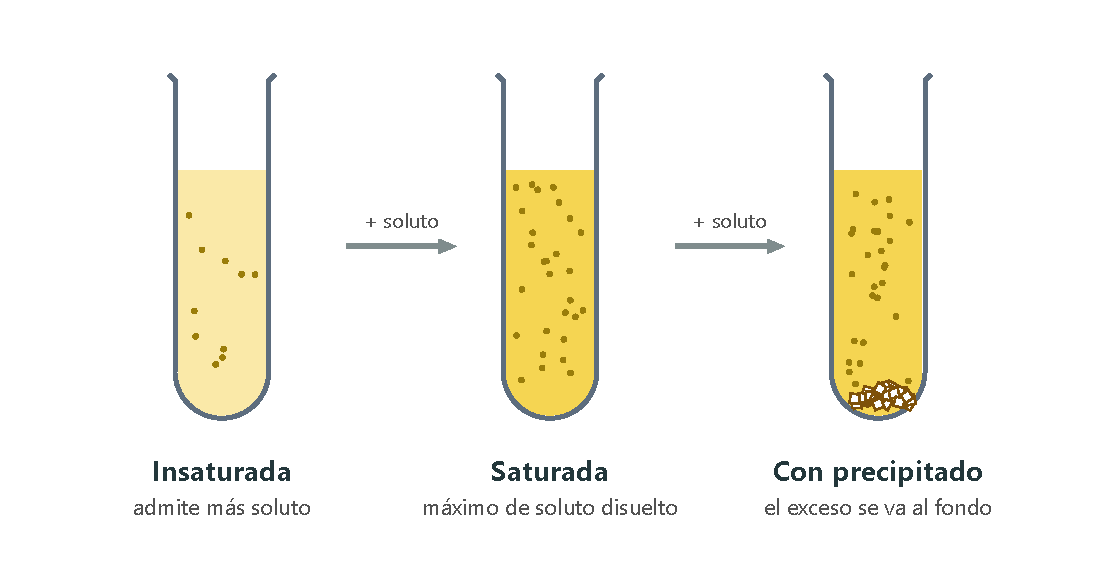
\includegraphics[width=0.6\textwidth]{images/UD2/saturacion}
    \caption{Al añadir soluto, una disolución pasa de insaturada a saturada; el soluto que sobra precipita.}
    \label{fig:ud2-saturacion}
\end{figure}

\subsection{Solubilidad y temperatura}

\paragraph{Sólidos en líquidos.} La \textbf{curva de solubilidad} representa la solubilidad de un soluto frente a la temperatura
(figura~\ref{fig:ud2-curvas}). En general, la solubilidad de los sólidos \textbf{aumenta} con la temperatura, aunque en algunos
casos apenas cambia (\ch{NaCl}) y en otros disminuye (\ch{Ce2(SO4)3}).

Si una disolución saturada en caliente se enfría, el soluto que ya no cabe precipita. El clorato de potasio, \ch{KClO3}, por
ejemplo, tiene una solubilidad de unos \qty{30}{\gram} en \qty{100}{\gram} de agua a \qty{70}{\degreeCelsius}, pero solo de
\qty{10}{\gram} a \qty{30}{\degreeCelsius}: al enfriar una disolución saturada que contenga \qty{100}{\gram} de agua, precipitan
unos \qty{20}{\gram} de \ch{KClO3}. Si el enfriamiento es muy lento y sin perturbaciones, puede que el exceso no precipite: se
obtiene una \textbf{disolución sobresaturada}, muy inestable; un golpe o un cristalito de soluto basta para que el exceso se separe,
a veces formando bonitos \textbf{cristales}.

\begin{figure}[H]
    \centering
    \begin{tikzpicture}
        \begin{axis}[grafica, width=0.7\linewidth, height=7.5cm,
            xlabel={Temperatura (\unit{\degreeCelsius})}, ylabel={Solubilidad (g / \qty{100}{\gram} de agua)},
            xmin=0, xmax=100, ymin=0, ymax=120, xtick={0,10,...,100}, ytick={0,20,...,120},
            clip=true, legend style={font=\scriptsize, at={(1.04,1)}, anchor=north west, cells={anchor=west}}]
            \addplot[thick, smooth, blue!70!black] coordinates {(0,13.3) (10,20.9) (20,31.6) (30,45.8) (40,63.9) (50,85.5) (60,110) (64,120)};
            \addplot[thick, smooth, green!50!black] coordinates {(0,59.5) (10,64.7) (20,74.5) (30,100) (40,116) (45,120)};
            \addplot[thick, smooth, orange!90!black] coordinates {(0,4.7) (10,7) (20,12) (30,20) (40,26) (50,34) (60,43) (70,52) (80,61) (90,70) (100,80)};
            \addplot[thick, smooth, red!70!black] coordinates {(0,28) (20,34.2) (40,40.1) (60,45.8) (80,51.3) (100,56.3)};
            \addplot[thick, smooth, violet] coordinates {(0,3.3) (10,5.2) (20,7.3) (30,10.1) (40,13.9) (50,19.3) (60,23.8) (70,30) (80,37.6) (90,46) (100,56.3)};
            \addplot[thick, smooth, black!70] coordinates {(0,35.7) (20,35.9) (40,36.4) (60,37.1) (80,38) (100,39.2)};
            \addplot[thick, smooth, brown!80!black] coordinates {(0,20) (10,15) (20,10) (30,7.2) (40,5.5) (60,3.8) (80,2.6) (100,2)};
            \legend{\ch{KNO3}, \ch{CaCl2}, \ch{K2Cr2O7}, \ch{KCl}, \ch{KClO3}, \ch{NaCl}, \ch{Ce2(SO4)3}}
        \end{axis}
    \end{tikzpicture}
    \caption{Curvas de solubilidad de algunas sales en agua (valores aproximados).}
    \label{fig:ud2-curvas}
\end{figure}

\paragraph{Gases en líquidos.} Cuando sacas un refresco de la nevera y lo sirves, se forman burbujas: al calentarse, el
\ch{CO2} disuelto escapa. La solubilidad de los \textbf{gases} en los líquidos \textbf{disminuye} al aumentar la temperatura
(figura~\ref{fig:ud2-gases}), porque las moléculas de gas, con más energía, escapan con más facilidad de la disolución.

\begin{figure}[H]
    \centering
    \begin{tikzpicture}
        \begin{axis}[grafica, width=0.48\linewidth, height=5cm,
            xlabel={\(t\) (\unit{\degreeCelsius})}, ylabel={\ch{CO2} disuelto (\unit{\gram\per\litre})},
            xmin=0, xmax=80, ymin=0, ymax=3.6, xtick={0,20,...,80}]
            \addplot[thick, smooth, red!75!black] coordinates {(0,3.35) (10,2.32) (20,1.69) (30,1.26) (40,0.97) (50,0.76) (60,0.58) (80,0.30)};
        \end{axis}
    \end{tikzpicture}
    \hfill
    \begin{tikzpicture}
        \begin{axis}[grafica, width=0.48\linewidth, height=5cm,
            xlabel={\(t\) (\unit{\degreeCelsius})}, ylabel={\ch{O2} disuelto (\unit{\milli\gram\per\litre})},
            xmin=0, xmax=40, ymin=0, ymax=16, xtick={0,10,...,40}]
            \addplot[thick, smooth, blue!70!black] coordinates {(0,14.6) (5,12.8) (10,11.3) (15,10.1) (20,9.1) (25,8.3) (30,7.6) (35,7.0) (40,6.4)};
        \end{axis}
    \end{tikzpicture}
    \caption{Solubilidad del dióxido de carbono (a \qty{1}{\atm} de \ch{CO2}) y del oxígeno (en contacto con el aire) en agua.}
    \label{fig:ud2-gases}
\end{figure}

\begin{example}
    \textbf{Lectura de las curvas de solubilidad.} Con la figura~\ref{fig:ud2-curvas}: a) compara la solubilidad del
    \ch{K2Cr2O7} a 20, 60 y \qty{80}{\degreeCelsius}; b) ¿qué es más soluble a \qty{20}{\degreeCelsius}, el \ch{CaCl2} o el
    \ch{KCl}? c) Se enfría hasta \qty{30}{\degreeCelsius} una disolución saturada de \ch{KClO3} a \qty{70}{\degreeCelsius} que
    contiene \qty{250}{\gram} de agua. ¿Cuánto soluto precipita?

    \textbf{Solución.} a) Unos \qty{12}{\gram}, \qty{43}{\gram} y \qty{61}{\gram} por \qty{100}{\gram} de agua: aumenta mucho
    con la temperatura, como en la mayoría de las sales. b) El \ch{CaCl2}: unos \qty{75}{\gram} frente a unos \qty{34}{\gram} de
    \ch{KCl}. c) En \qty{100}{\gram} de agua precipitan \(30 - 10 = \qty{20}{\gram}\); en \qty{250}{\gram},
    \(20 \cdot \num{2.5} = \qty{50}{\gram}\) de \ch{KClO3}.
\end{example}

\begin{example}
    \textbf{Vertidos de agua caliente.} Una empresa vierte agua caliente a un río. ¿Cómo afecta a los peces?

    \textbf{Solución.} Los peces respiran el oxígeno disuelto en el agua. Al aumentar la temperatura disminuye la solubilidad del
    oxígeno (figura~\ref{fig:ud2-gases}): a \qty{30}{\degreeCelsius} el agua disuelve casi la mitad que a \qty{0}{\degreeCelsius}.
    Esta \textbf{contaminación térmica} deja menos oxígeno disponible, y los peces pueden morir asfixiados.
\end{example}

\subsection{Solubilidad de los gases y presión}

La presión apenas influye en la solubilidad de sólidos y líquidos, pero mucho en la de los gases. Las moléculas de un gas chocan
contra la superficie del líquido; si la presión aumenta, hay más choques y se disuelven más moléculas hasta alcanzar un nuevo
equilibrio (figura~\ref{fig:ud2-henry}). \textbf{William Henry} (1775-1836) recogió este comportamiento en una ley:

\begin{definition}[Ley de Henry]
    A temperatura constante, la solubilidad de un gas en un líquido es directamente proporcional a la presión parcial del gas
    sobre la disolución:
    \[ c = k \, p \]
    La constante \(k\) depende del gas, del disolvente y de la temperatura (por ejemplo, en \unit{\mol\per\litre\per\atm}).
\end{definition}

\begin{figure}[H]
    \centering
    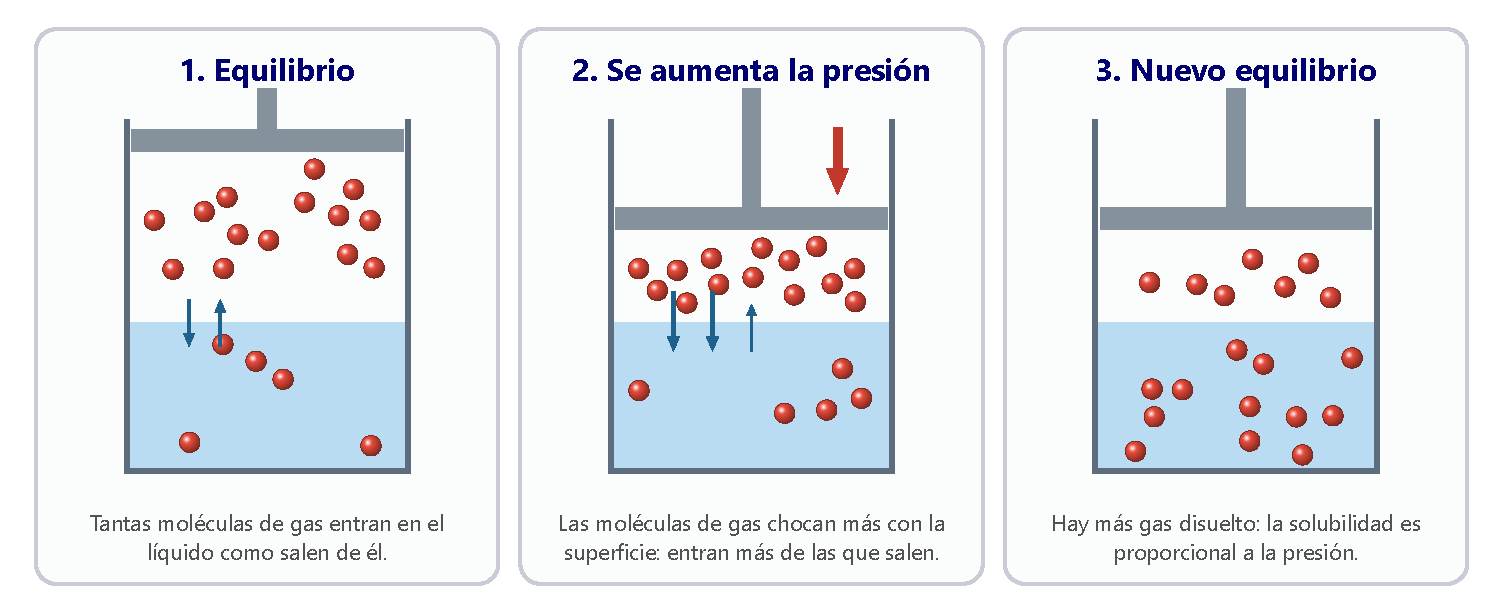
\includegraphics[width=0.95\textwidth]{images/UD2/henry}
    \caption{Al aumentar la presión de un gas sobre un líquido, aumenta la cantidad de gas disuelto.}
    \label{fig:ud2-henry}
\end{figure}

Por eso los refrescos se envasan con \ch{CO2} a varias atmósferas: al abrirlos, la presión de \ch{CO2} baja bruscamente y el
gas sobrante escapa en forma de burbujas. La ley de Henry también explica los problemas de los buceadores: a gran profundidad
respiran aire a alta presión y se disuelve mucho nitrógeno en la sangre; si suben deprisa, el gas forma burbujas
(enfermedad descompresiva).

\begin{example}
    \textbf{Nitrógeno disuelto.} Un recipiente contiene \qty{5}{\litre} de agua en contacto con aire a una presión total de
    \qty{3}{\atm}. La fracción molar del nitrógeno en el aire es \num{0.78} y su constante de Henry en agua, a esa temperatura,
    es \qty{6.4e-4}{\mol\per\litre\per\atm}. ¿Qué masa de nitrógeno hay disuelta?

    \textbf{Solución.} Presión parcial del nitrógeno: \(p(\ch{N2}) = \chi \, p_T = \num{0.78} \cdot 3 = \qty{2.34}{\atm}\).
    \[ c = k \, p = \num{6.4e-4} \cdot \num{2.34} = \qty{1.50e-3}{\mol\per\litre}; \qquad
    m = \qty{1.50e-3}{\mol\per\litre} \cdot \qty{5}{\litre} \cdot \qty{28}{\gram\per\mol} = \qty{0.21}{\gram} \]
\end{example}

\begin{exercise}
    La constante de Henry del oxígeno en agua a \qty{20}{\degreeCelsius} es \qty{1.3e-3}{\mol\per\litre\per\atm}. ¿Cuántos
    miligramos de oxígeno hay disueltos en \qty{2}{\litre} de agua en contacto con aire a \qty{1}{\atm} (21\,\% de \ch{O2})?
    \begin{solu}
        \(p(\ch{O2}) = \qty{0.21}{\atm}\); \(c = \num{1.3e-3} \cdot \num{0.21} = \qty{2.73e-4}{\mol\per\litre}\);
        \(m = \num{2.73e-4} \cdot 2 \cdot 32 = \qty{0.0175}{\gram} = \textcolor{red}{\qty{17.5}{\milli\gram}}\).
    \end{solu}
\end{exercise}

\begin{exercise}
    Explica por qué: a) un refresco pierde antes el gas si está caliente; b) en verano, en los estanques con poca agua, los peces
    suben a la superficie a «boquear».
    \begin{solu}
        a) \textcolor{red}{La solubilidad del \ch{CO2} disminuye al aumentar la temperatura}. b) \textcolor{red}{El agua caliente
        disuelve menos oxígeno}, y los peces buscan la superficie, donde el agua está en contacto con el aire.
    \end{solu}
\end{exercise}

%========================================================================================
\section{Propiedades coligativas}\label{sec:ud2-coligativas}
%========================================================================================

En invierno se echa sal en las carreteras para que no se forme hielo; al cocer pasta, el agua con sal hierve a algo más de
\qty{100}{\degreeCelsius}; y muchos alimentos se conservan en salmuera o en almíbar. Todos estos fenómenos se deben a que las
propiedades físicas de una disolución son diferentes de las del disolvente puro. Hay dos tipos de propiedades:

\begin{itemize}
    \item \textbf{Propiedades constitutivas}: dependen de la naturaleza de los componentes (densidad, viscosidad, color).
    \item \textbf{Propiedades coligativas}: dependen solo del \textbf{número de partículas} de soluto (de su concentración), y no
    de cuál sea el soluto. Son cuatro: el \textbf{descenso de la presión de vapor}, el \textbf{aumento del punto de ebullición}, el
    \textbf{descenso del punto de congelación} y la \textbf{presión osmótica}.
\end{itemize}

\subsection{Descenso de la presión de vapor}

En un líquido, algunas partículas tienen energía suficiente para escapar de la superficie y pasar a gas (\textbf{evaporación}).
En un recipiente cerrado, las partículas del vapor también chocan con la superficie y vuelven al líquido
(\textbf{condensación}). Al cabo de un tiempo se alcanza un \textbf{equilibrio dinámico}: se evaporan tantas partículas como
se condensan. La \textbf{presión de vapor} es la presión del vapor en equilibrio con su líquido; depende de la sustancia y aumenta
con la temperatura. Cuando la presión de vapor iguala la presión exterior, el líquido hierve.

Si se añade un \textbf{soluto no volátil} (que no pasa a vapor), parte de la superficie la ocupan partículas de soluto y menos
moléculas de disolvente pueden escapar: \textbf{la presión de vapor disminuye} (figura~\ref{fig:ud2-presion-vapor}).

\begin{figure}[H]
    \centering
    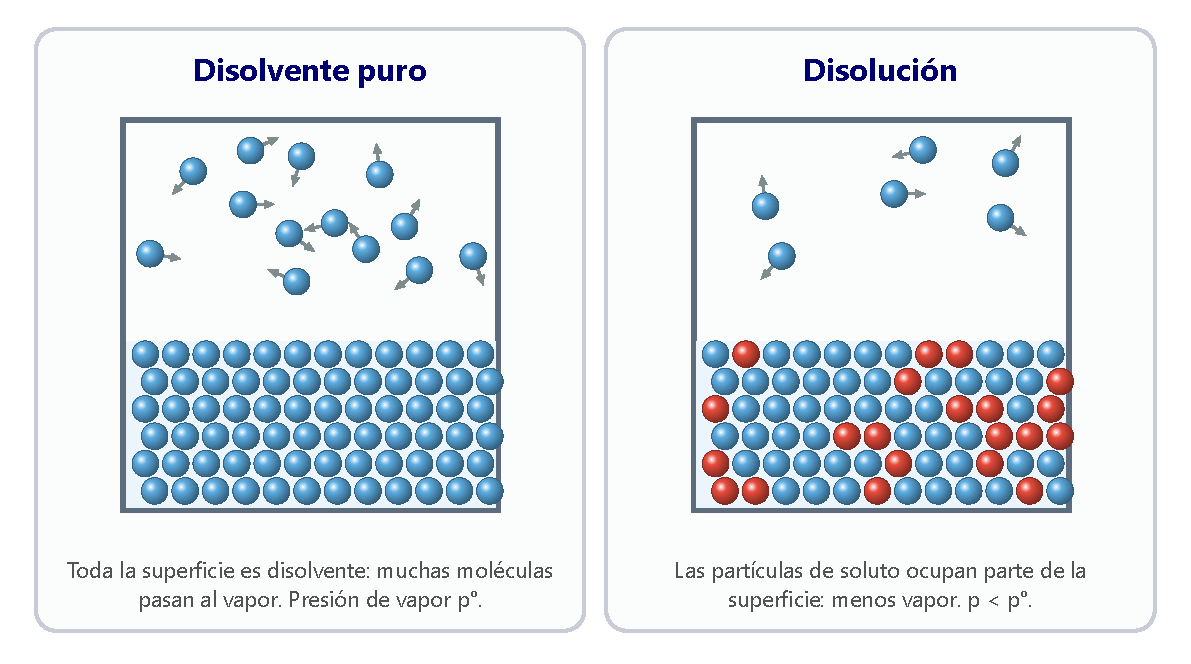
\includegraphics[width=0.75\textwidth]{images/UD2/presion_vapor}
    \caption{Un soluto no volátil hace que menos moléculas de disolvente pasen al vapor.}
    \label{fig:ud2-presion-vapor}
\end{figure}

\textbf{François-Marie Raoult} (1830-1901) midió este efecto y lo resumió en una ley:

\begin{definition}[Ley de Raoult]
    A una temperatura dada, la disminución de la presión de vapor de un disolvente al añadirle un soluto no volátil es
    proporcional a la fracción molar del soluto:
    \[ \Delta p = p^{\circ} - p = p^{\circ} \chi_s \qquad \text{o, lo que es lo mismo,} \qquad p = p^{\circ} \chi_d \]
    \(p^{\circ}\) es la presión de vapor del disolvente puro, \(p\) la de la disolución, \(\chi_s\) la fracción molar del soluto y
    \(\chi_d\) la del disolvente. Las disoluciones que cumplen exactamente esta ley se llaman \textbf{disoluciones ideales}.
\end{definition}

\begin{example}
    \textbf{Presión de vapor de una disolución de glicerina.} La presión de vapor del agua a \qty{25}{\degreeCelsius} es
    \qty{23.8}{\mmHg}. Se disuelven \qty{46}{\gram} de glicerina, \ch{C3H8O3} (no volátil), en \qty{180}{\gram} de agua.
    Calcula la presión de vapor de la disolución.

    \textbf{Solución.} \(n_{\text{glicerina}} = \dfrac{46}{92} = \qty{0.5}{\mol}\); \(n_{\text{agua}} = \dfrac{180}{18} = \qty{10}{\mol}\);
    \(\chi_s = \dfrac{\num{0.5}}{\num{10.5}} = \num{0.0476}\).
    \[ \Delta p = p^{\circ} \chi_s = \num{23.8} \cdot \num{0.0476} = \qty{1.13}{\mmHg}; \qquad p = \num{23.8} - \num{1.13} = \qty{22.7}{\mmHg} \]
\end{example}

\begin{exercise}
    La presión de vapor del etanol a \qty{50}{\degreeCelsius} es \qty{221.6}{\mmHg}. Se disuelven \qty{20}{\gram} de urea,
    \ch{CO(NH2)2}, en \qty{150}{\mL} de etanol (\(d = \qty{0.79}{\gram\per\mL}\)). ¿Cuál es la presión de vapor de la
    disolución a esa temperatura?
    \begin{solu}
        \(n_{\text{urea}} = 20/60 = \qty{0.333}{\mol}\); \(n_{\text{etanol}} = \num{118.5}/46 = \qty{2.58}{\mol}\);
        \(\chi_s = \num{0.115}\): \(\Delta p = \qty{25.4}{\mmHg}\); \(p = \textcolor{red}{\qty{196}{\mmHg}}\).
    \end{solu}
\end{exercise}

\subsection{Aumento del punto de ebullición y descenso del punto de congelación}

Como la disolución tiene menor presión de vapor, hay que calentarla más para que su presión de vapor llegue a igualar la presión
atmosférica: \textbf{la disolución hierve a una temperatura más alta} que el disolvente puro. Del mismo modo, las partículas de
soluto dificultan que las de disolvente se ordenen para formar el sólido: \textbf{la disolución congela a una temperatura más
baja} (figura~\ref{fig:ud2-diagrama}).

\begin{figure}[H]
    \centering
    \begin{tikzpicture}
        \begin{axis}[grafica, width=0.75\linewidth, height=6cm,
            xlabel={Temperatura}, ylabel={Presión de vapor},
            xmin=60, xmax=118, ymin=0, ymax=1.5, xtick=\empty, ytick={1}, yticklabels={\qty{1}{\atm}}, grid=none]
            \addplot[thick, blue!70!black, domain=60:116] {10^(8.07131 - 1730.63/(233.426 + x))/760};
            \addplot[thick, red!75!black, domain=60:116] {0.88*10^(8.07131 - 1730.63/(233.426 + x))/760};
            \addplot[dashed, gray] coordinates {(60,1) (118,1)};
            \addplot[dashed, gray] coordinates {(100,1) (100,0)};
            \addplot[dashed, gray] coordinates {(103.6,1) (103.6,0)};
            \draw[<->, thick] (axis cs:100,0.12) -- node[below, font=\small] {\(\Delta T_e\)} (axis cs:103.6,0.12);
            \draw[<->, thick] (axis cs:85,0.574) -- node[right, font=\small] {\(\Delta p\)} (axis cs:85,0.505);
            \node[font=\small, blue!70!black, anchor=east] at (axis cs:110,1.38) {disolvente puro};
            \node[font=\small, red!75!black, anchor=west] at (axis cs:110,1.0) {disolución};
            \node[font=\scriptsize, anchor=north] at (axis cs:100,0) {\(T_e\)};
            \node[font=\scriptsize, anchor=north] at (axis cs:104.4,0) {\(T_e'\)};
        \end{axis}
    \end{tikzpicture}
    \caption{La curva de presión de vapor de la disolución queda por debajo de la del disolvente: hierve a mayor temperatura.}
    \label{fig:ud2-diagrama}
\end{figure}

\begin{definition}[Ascenso ebulloscópico y descenso crioscópico]
    Para disoluciones diluidas de solutos no volátiles, las variaciones de las temperaturas de ebullición y de congelación son
    proporcionales a la \textbf{molalidad}:
    \[ \Delta T_e = T_e' - T_e = K_e \, m \qquad\qquad \Delta T_c = T_c - T_c' = K_c \, m \]
    \(T_e\) y \(T_c\) son las temperaturas del disolvente puro, y \(T_e'\) y \(T_c'\), las de la disolución. \(K_e\) es la
    \textbf{constante ebulloscópica} y \(K_c\) la \textbf{constante crioscópica}; dependen solo del disolvente.
\end{definition}

\begin{table}[H]
    \centering
    \caption{Constantes ebulloscópicas y crioscópicas de algunos disolventes (a \qty{1}{\atm})}
    \vspace{-5pt}
    \begin{tabular}{@{}lcccc@{}}
        \toprule
        \textbf{Disolvente} & \makecell{\(T_e\) \\ (\unit{\degreeCelsius})} & \makecell{\(K_e\) \\ (\unit{\degreeCelsius\kilo\gram\per\mol})} &
        \makecell{\(T_c\) \\ (\unit{\degreeCelsius})} & \makecell{\(K_c\) \\ (\unit{\degreeCelsius\kilo\gram\per\mol})} \\
        \midrule
        Agua & 100 & \num{0.52} & 0 & \num{1.86} \\[3pt]
        Benceno & \num{80.1} & \num{2.53} & \num{5.5} & \num{5.12} \\[3pt]
        Ciclohexano & \num{80.7} & \num{2.79} & \num{6.5} & \num{20.1} \\[3pt]
        Tetracloruro de carbono & \num{76.5} & \num{4.95} & \num{-22.3} & \num{29.8} \\[3pt]
        Cloroformo & \num{61.2} & \num{3.63} & \num{-63.5} & \num{4.68} \\[3pt]
        Etanol & \num{78.4} & \num{1.19} & \num{-114.6} & \num{1.99} \\[3pt]
        Alcanfor & 204 & \num{5.95} & 178 & 40 \\
        \bottomrule
    \end{tabular}
    \label{tab:ud2-constantes}
\end{table}

Estas propiedades tienen muchas aplicaciones: los \textbf{anticongelantes} (etilenglicol) del circuito de refrigeración de los
coches, la sal en las carreteras heladas o la mezcla de hielo y sal para enfriar rápidamente. Además, midiendo \(\Delta T\) se
puede calcular la \textbf{masa molar} de un soluto desconocido.

\begin{remark}
    \textbf{Solutos iónicos.} Las propiedades coligativas dependen del número de partículas. Un soluto iónico se disocia: cada
    unidad de \ch{NaCl} da dos iones (\ch{Na+} y \ch{Cl-}) y cada una de \ch{CaCl2}, tres. Por eso su efecto se multiplica por un
    factor \(i\), el \textbf{factor de van't Hoff} (\(i \approx 2\) para el \ch{NaCl}): \(\Delta T_c = i \, K_c \, m\). En los
    ejercicios de esta unidad, salvo que se diga lo contrario, los solutos son moleculares (\(i = 1\)).
\end{remark}

\begin{example}
    \textbf{Masa molar por ebulloscopia.} Al disolver \qty{9}{\gram} de una sustancia desconocida en \qty{150}{\gram} de agua,
    la temperatura de ebullición aumenta \qty{0.26}{\degreeCelsius}. Calcula la masa molar del soluto.

    \textbf{Solución.} \(m = \dfrac{\Delta T_e}{K_e} = \dfrac{\num{0.26}}{\num{0.52}} = \qty{0.5}{\mol\per\kilo\gram}\).
    Moles de soluto: \(n = m \cdot m_{\text{disolvente}} = \num{0.5} \cdot \num{0.150} = \qty{0.075}{\mol}\).
    \[ M = \frac{\qty{9}{\gram}}{\qty{0.075}{\mol}} = \qty{120}{\gram\per\mol} \]
\end{example}

\begin{example}
    \textbf{Congelación del ciclohexano.} Calcula la temperatura de congelación de una disolución de \qty{6.4}{\gram} de
    naftaleno, \ch{C10H8}, en \qty{100}{\gram} de ciclohexano.

    \textbf{Solución.} \(M(\ch{C10H8}) = \qty{128}{\gram\per\mol}\); \(m = \dfrac{\num{6.4}/128}{\num{0.1}} = \qty{0.5}{\mol\per\kilo\gram}\).
    \(\Delta T_c = K_c \, m = \num{20.1} \cdot \num{0.5} = \qty{10.05}{\degreeCelsius}\);
    \(T_c' = \num{6.5} - \num{10.05} = \qty{-3.55}{\degreeCelsius}\).
\end{example}

\begin{exercise}
    La temperatura de ebullición del etanol es \qty{78.4}{\degreeCelsius}. Si disolvemos \qty{30}{\gram} de urea,
    \ch{CO(NH2)2}, en \qty{200}{\gram} de etanol, ¿a qué temperatura hervirá la disolución?
    \begin{solu}
        \(m = \dfrac{\num{0.5}}{\num{0.2}} = \qty{2.5}{\mol\per\kilo\gram}\); \(\Delta T_e = \num{1.19} \cdot \num{2.5} = \qty{2.98}{\degreeCelsius}\):
        \(T_e' = \textcolor{red}{\qty{81.4}{\degreeCelsius}}\).
    \end{solu}
\end{exercise}

\begin{exercise}
    ¿Qué masa de maltosa, \ch{C12H22O11}, hay que disolver en \qty{250}{\gram} de agua para que su temperatura de ebullición
    aumente \qty{0.4}{\degreeCelsius}?
    \begin{solu}
        \(m = \num{0.4}/\num{0.52} = \qty{0.769}{\mol\per\kilo\gram}\); \(n = \num{0.769} \cdot \num{0.25} = \qty{0.192}{\mol}\):
        \(\textcolor{red}{\qty{65.8}{\gram}}\) de maltosa.
    \end{solu}
\end{exercise}

\begin{exercise}
    a) ¿Por qué en las zonas de montaña el agua hierve a menos de \qty{100}{\degreeCelsius}? b) ¿Por qué se echa sal en las
    carreteras heladas, y por qué no sirve cuando hace mucho frío (por debajo de unos \qty{-20}{\degreeCelsius})?
    \begin{solu}
        a) \textcolor{red}{La presión atmosférica es menor}, y la presión de vapor del agua la iguala a menor temperatura (en la
        cima del Everest, a unos \qty{70}{\degreeCelsius}). b) \textcolor{red}{La sal disuelta baja el punto de congelación del
        agua}, de modo que el hielo funde aunque la temperatura sea menor que \qty{0}{\degreeCelsius}; pero ese descenso tiene un
        límite (el de la disolución saturada, unos \qty{-21}{\degreeCelsius}).
    \end{solu}
\end{exercise}

\subsection{Presión osmótica}

Una \textbf{membrana semipermeable} deja pasar las moléculas de disolvente, pero no las de soluto. Si separa dos disoluciones de
distinta concentración, el disolvente pasa de la \textbf{más diluida a la más concentrada}, hasta que las concentraciones se
igualan o el nivel que sube compensa el proceso (figura~\ref{fig:ud2-osmosis}). Este fenómeno se llama \textbf{ósmosis} y es
fundamental en biología: así se intercambia agua a través de las membranas de las células.

\begin{definition}[Presión osmótica]
    Es la presión, \(\pi\), que hay que ejercer sobre la disolución más concentrada para impedir el paso neto de disolvente a través
    de la membrana. \textbf{Van't Hoff} (1852-1911) descubrió que, en disoluciones diluidas, cumple una ecuación igual a la de los
    gases ideales:
    \[ \pi V = n R T \quad \Rightarrow \quad \pi = \frac{n}{V} R T = c \, R \, T \]
    donde \(c\) es la concentración molar y \(T\), la temperatura absoluta.
\end{definition}

\begin{figure}[H]
    \centering
    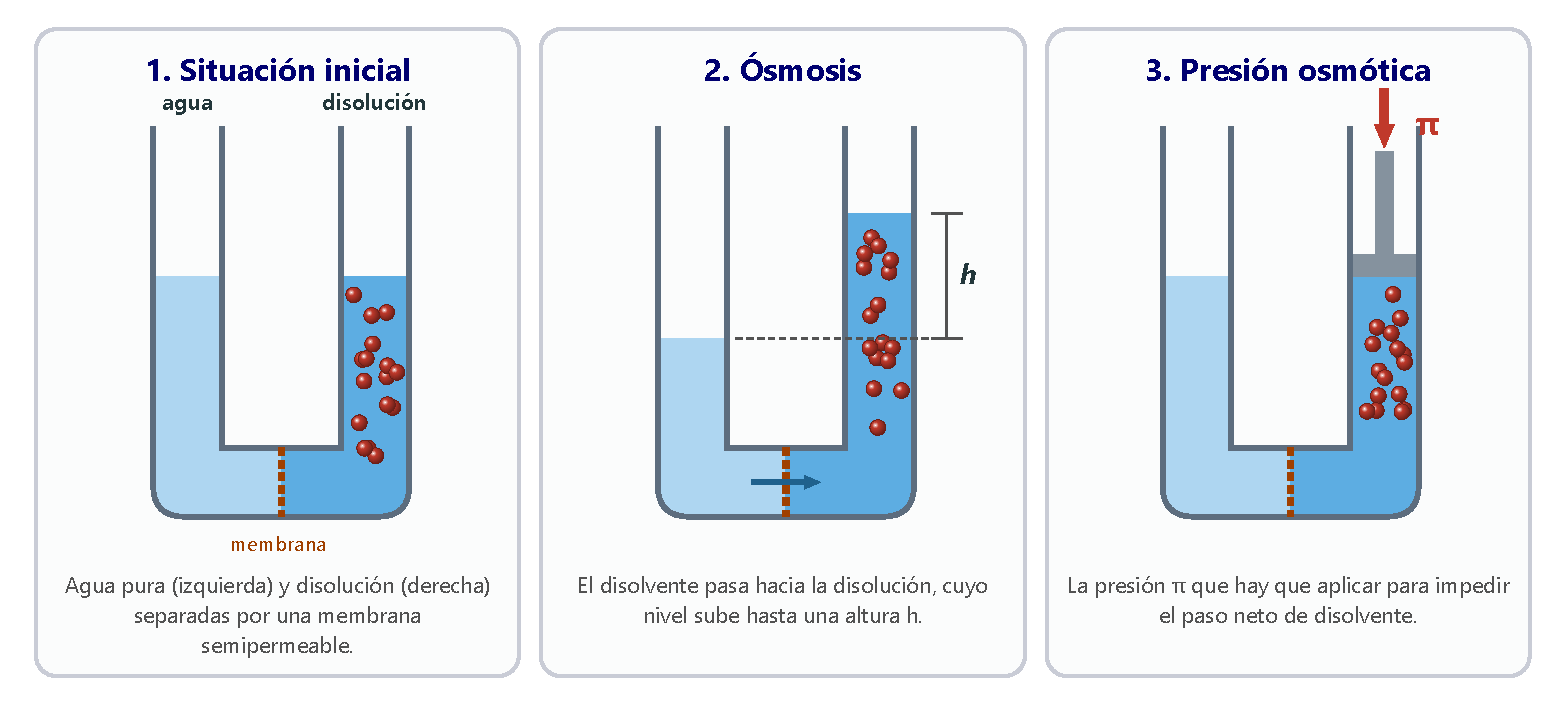
\includegraphics[width=0.95\textwidth]{images/UD2/osmosis}
    \caption{Ósmosis y presión osmótica.}
    \label{fig:ud2-osmosis}
\end{figure}

La presión osmótica es fácil de medir y alcanza valores grandes incluso con concentraciones pequeñas; por eso se usa para
determinar masas molares de sustancias de masa molar muy alta, como las proteínas.

\paragraph{Disoluciones isotónicas, hipertónicas e hipotónicas.} Dos disoluciones con la misma presión osmótica son
\textbf{isotónicas}. Si una tiene mayor presión osmótica que otra de referencia, es \textbf{hipertónica}; si la tiene menor,
\textbf{hipotónica}. Las células se comportan de forma distinta según el medio que las rodea (figura~\ref{fig:ud2-tonicidad}):
en un medio hipertónico pierden agua y se arrugan; en uno hipotónico, la ganan y pueden llegar a romperse. Por eso los sueros y
los medicamentos inyectables son disoluciones isotónicas con la sangre.

\begin{figure}[H]
    \centering
    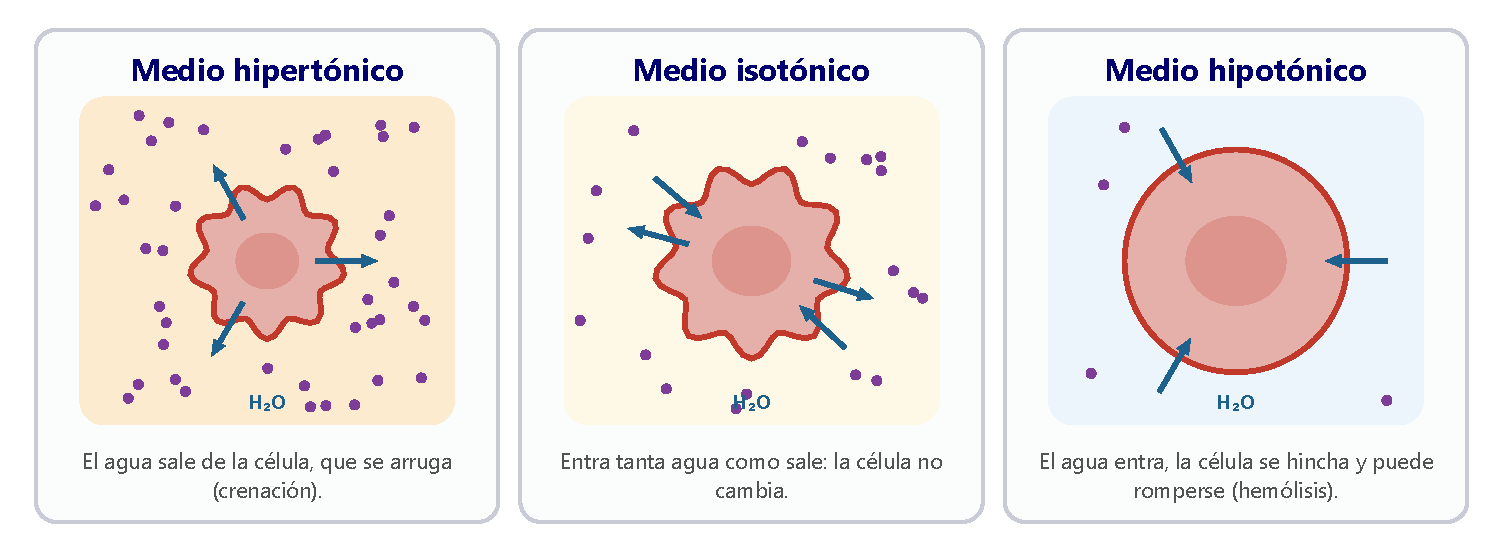
\includegraphics[width=0.95\textwidth]{images/UD2/tonicidad}
    \caption{Glóbulos rojos en disoluciones hipertónica, isotónica e hipotónica.}
    \label{fig:ud2-tonicidad}
\end{figure}

\paragraph{Ósmosis inversa.} Si sobre la disolución más concentrada se aplica una presión \textbf{mayor} que la osmótica, el
disolvente pasa en sentido contrario, de la disolución concentrada a la diluida. Es la \textbf{ósmosis inversa}, que usan las
plantas \textbf{desaladoras} para obtener agua potable a partir de agua de mar (figura~\ref{fig:ud2-inversa}) y muchos
purificadores domésticos.

\begin{figure}[H]
    \centering
    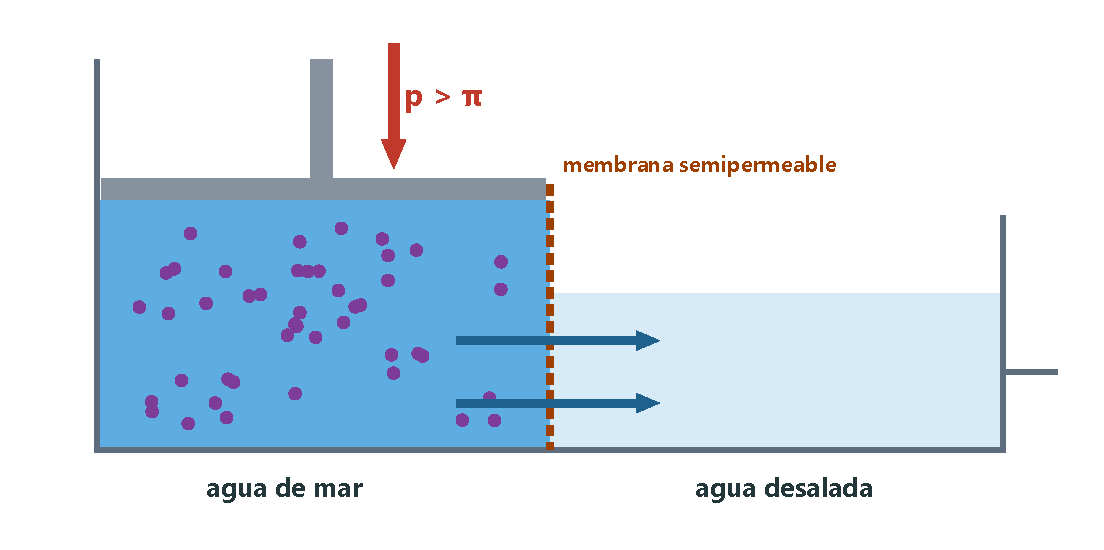
\includegraphics[width=0.65\textwidth]{images/UD2/osmosis_inversa}
    \caption{Ósmosis inversa en una planta desaladora.}
    \label{fig:ud2-inversa}
\end{figure}

\begin{example}
    \textbf{Presión osmótica y masa molar.} a) Calcula la presión osmótica de una disolución de glucosa \qty{0.3}{\mol\per\litre}
    a \qty{37}{\degreeCelsius}. b) Una disolución de \qty{250}{\mL} que contiene \qty{4}{\gram} de un soluto desconocido tiene,
    a \qty{25}{\degreeCelsius}, una presión osmótica de \qty{3000}{\mmHg}. ¿Cuál es la masa molar del soluto?

    \textbf{Solución.} a) \(\pi = c R T = \num{0.3} \cdot \num{0.082} \cdot 310 = \qty{7.63}{\atm}\).

    b) \(\pi = \dfrac{3000}{760} = \qty{3.95}{\atm}\). De \(\pi V = \dfrac{m}{M} R T\):
    \[ M = \frac{m R T}{\pi V} = \frac{4 \cdot \num{0.082} \cdot 298}{\num{3.95} \cdot \num{0.25}} = \qty{99}{\gram\per\mol} \]
\end{example}

\begin{example}
    \textbf{¿Por qué no podemos beber agua de mar?}

    \textbf{Solución.} El agua de mar tiene una concentración de sales mucho mayor que la de nuestros líquidos corporales: es un
    medio \textbf{hipertónico}. Al beberla, las células tienden a igualar concentraciones cediendo agua por ósmosis; además, los
    riñones necesitan más agua para eliminar el exceso de sal de la que se ha bebido. El resultado es que nos
    \textbf{deshidratamos}.
\end{example}

\begin{exercise}
    Investiga qué técnicas de conservación de alimentos se basan en la presión osmótica (salazón, almíbar, salmuera…). ¿Por qué
    la lechuga aliñada con sal se ablanda al cabo de un rato?
    \begin{solu}
        \textcolor{red}{En un medio muy concentrado (hipertónico), los microorganismos pierden agua por ósmosis y no pueden
        crecer}: así se conservan las salazones, las mermeladas o las frutas en almíbar. \textcolor{red}{La sal forma una disolución
        hipertónica sobre la lechuga}: sus células pierden agua y la hoja se arruga y se ablanda.
    \end{solu}
\end{exercise}

\begin{exercise}
    Los riñones filtran la sangre para eliminar sustancias de desecho. Cuando fallan, los pacientes se someten a
    \textbf{diálisis}. Investiga en qué consiste y en qué se parece a la ósmosis.
    \begin{solu}
        \textcolor{red}{En la diálisis la sangre circula junto a un líquido de diálisis, separados por una membrana semipermeable}
        con poros que dejan pasar el agua y las moléculas pequeñas (urea, sales en exceso), pero no las células ni las proteínas.
        Los desechos pasan de la sangre, donde están más concentrados, al líquido de diálisis. Se parece a la ósmosis en el uso de
        la membrana, pero en la diálisis atraviesan la membrana \textbf{solutos}, no solo el disolvente.
    \end{solu}
\end{exercise}

%========================================================================================
\section{Química en la vida: cómo limpiar la casa con productos de la cocina}\label{sec:ud2-limpieza}
%========================================================================================

Muchos productos de limpieza son disoluciones de sustancias contaminantes que, en ocasiones, podemos sustituir por otras más
sencillas. Algunos ejemplos:

\begin{itemize}
    \item \textbf{Superficies metálicas oxidadas}: unas gotas de \textbf{zumo de limón} o de pomelo. Su ácido cítrico reacciona con
    los óxidos y los convierte en sales solubles en agua.
    \item \textbf{Parrilla del horno con óxido}: frotarla con media \textbf{cebolla}. Al frotar se libera agua con aminoácidos y
    enzimas que ayudan a disolver los óxidos adheridos.
    \item \textbf{Suelos de madera}: un poco de \textbf{té negro} en el agua de fregar. El té contiene \textbf{taninos}, los mismos
    que hay en la corteza de los árboles, que desinfectan y devuelven el color a la madera.
    \item \textbf{Baño}: \textbf{vinagre}, una disolución acuosa de ácido acético (en torno al 5\,\%). Disuelve la cal y, al ser
    ácido, impide que crezcan muchos microorganismos.
\end{itemize}

\begin{exercise}
    a) El vinagre de limpieza tiene un 6\,\% en masa de ácido acético, \ch{CH3COOH}, y una densidad de \qty{1.01}{\gram\per\mL}.
    Calcula su concentración molar. b) ¿Por qué el vinagre elimina la cal (carbonato de calcio) de los grifos? c) ¿Qué ventaja
    ambiental tiene usar estos productos?
    \begin{solu}
        a) \(c = \dfrac{\num{0.06} \cdot 1010}{60} = \textcolor{red}{\qty{1.01}{\mol\per\litre}}\). b) \textcolor{red}{Porque el
        ácido reacciona con el carbonato de calcio} y forma acetato de calcio, soluble en agua, y dióxido de carbono.
        c) \textcolor{red}{Son biodegradables, baratos y no contaminan el agua} con tensioactivos, fosfatos o disolventes.
    \end{solu}
\end{exercise}

%========================================================================================
\section{Prácticas}\label{sec:ud2-practicas}
%========================================================================================

\subsection{Preparación de una disolución de sulfato de cobre(II)}

\begin{multicols}{2}
    \textbf{Objetivo}
    \begin{itemize}
        \item Preparar \qty{250}{\mL} de una disolución de \ch{CuSO4} \qty{0.1}{\mol\per\litre} y, a partir de ella, otra diluida.
    \end{itemize}
    \columnbreak
    \textbf{Material y reactivos}
    \begin{itemize}
        \item Balanza, vidrio de reloj, espátula, vaso de precipitados, varilla, embudo, frasco lavador, cuentagotas, pipeta
        con aspirador y matraces aforados de 250 y \qty{100}{\mL}.
        \item Sulfato de cobre(II) anhidro y agua destilada.
    \end{itemize}
\end{multicols}

\textbf{Procedimiento}
\begin{enumerate}[label=\numberballgreen]
    \item Calcula la masa de \ch{CuSO4} necesaria (ejemplo de la sección~\ref{sec:ud2-preparacion}) y prepara la disolución siguiendo
    los pasos de la figura~\ref{fig:ud2-prep-solido}. \textbf{Usa guantes y gafas: el sulfato de cobre es nocivo.}
    \item Calcula el volumen de esa disolución que necesitas para preparar \qty{100}{\mL} de disolución
    \qty{0.02}{\mol\per\litre}. Tómalo con la pipeta, viértelo en el matraz de \qty{100}{\mL} y enrasa.
    \item Compara el color de las dos disoluciones y etiquétalas.
\end{enumerate}

\begin{exercise}
    a) ¿Qué volumen de la disolución \qty{0.1}{\mol\per\litre} necesitas en el paso 2? b) ¿Por qué el color de la disolución
    diluida es más claro? c) Si al enrasar el menisco queda por encima de la marca, ¿la concentración será mayor o menor que la
    calculada?
    \begin{solu}
        a) \(V_1 = \dfrac{\num{0.02} \cdot 100}{\num{0.1}} = \textcolor{red}{\qty{20}{\mL}}\). b) \textcolor{red}{Hay menos iones
        \ch{Cu^2+} (responsables del color azul) por unidad de volumen}. c) \textcolor{red}{Menor}: el mismo soluto ocupa un volumen
        mayor.
    \end{solu}
\end{exercise}

\subsection{¿Cómo enfriar una lata de refresco en menos de diez minutos?}

\begin{multicols}{2}
    \textbf{Objetivo}
    \begin{itemize}
        \item Comprobar el descenso del punto de congelación del agua al añadir sal o alcohol.
    \end{itemize}
    \columnbreak
    \textbf{Material}
    \begin{itemize}
        \item Tres cuencos grandes, tres latas iguales de la misma bebida, hielo picado, sal, \qty{100}{\mL} de alcohol y un
        termómetro.
    \end{itemize}
\end{multicols}

\textbf{Procedimiento}
\begin{enumerate}[label=\numberballgreen]
    \item \textbf{Cuenco 1}: un puñado de hielo picado que cubra el fondo y un poco de agua.
    \item \textbf{Cuenco 2}: la misma cantidad de hielo y agua, y un buen puñado de sal.
    \item \textbf{Cuenco 3}: la misma cantidad de hielo, \qty{100}{\mL} de agua y \qty{100}{\mL} de alcohol.
    \item Introduce una lata en cada cuenco, espera diez minutos y mide la temperatura de cada mezcla y de cada bebida.
\end{enumerate}

\begin{exercise}
    a) ¿En qué cuencos baja más la temperatura? ¿Por qué? b) ¿Qué propiedad coligativa explica el experimento? c) Cita otra
    situación cotidiana en la que se use para enfriar o descongelar algo.
    \begin{solu}
        a) \textcolor{red}{En los cuencos 2 y 3}: la sal o el alcohol disueltos bajan el punto de congelación del agua; el hielo
        sigue fundiendo por debajo de \qty{0}{\degreeCelsius} y, para fundir, toma calor de la mezcla y de la lata, que se enfrían
        mucho más que con hielo solo. b) \textcolor{red}{El descenso crioscópico}. c) \textcolor{red}{Echar sal en las carreteras
        heladas, los anticongelantes de los coches} o las heladeras artesanas de hielo y sal.
    \end{solu}
\end{exercise}

%========================================================================================
\section{Situación de aprendizaje: agua limpia y saneamiento (ODS 6)}\label{sec:ud2-ods}
%========================================================================================

El \textbf{Objetivo de Desarrollo Sostenible 6} busca garantizar el acceso de todas las personas al agua potable y al
saneamiento, y una gestión sostenible del agua. España es uno de los países europeos más amenazados por la sequía: los expertos
advierten de que, con el calentamiento global, los periodos secos serán cada vez más largos. Algunas empresas de abastecimiento
calculan que cada persona gasta en casa unos \qty{140}{\litre} de agua al día, y se ha propuesto reducir ese consumo a unos
\qty{100}{\litre}.

\begin{marker}
    \textbf{Reto:} calculad vuestro consumo de agua y vuestra huella hídrica, y proponed medidas para reducirlos.
\end{marker}

\begin{enumerate}[label=\numberballred]
    \item \textbf{¿Cuánta agua consumes cada día?} Estima tu consumo con estos datos aproximados: grifo abierto, \qty{12}{\litre}
    por minuto; ducha, \qty{60}{\litre} en 5 minutos; cisterna, de 6 a \qty{12}{\litre} por descarga; lavar los platos a mano con
    el grifo abierto, unos \qty{100}{\litre}. ¿Qué acciones podrías cambiar para reducirlo?
    \item \textbf{Huella hídrica.} El agua que gastamos no es solo la del grifo: también la que se usa para producir lo que
    comemos o vestimos. Por ejemplo, producir \qty{1}{\kilo\gram} de carne de ternera requiere unos \qty{15000}{\litre};
    \qty{1}{\kilo\gram} de chocolate, unos \qty{17000}{\litre}; unos pantalones vaqueros, unos \qty{8000}{\litre}; y
    \qty{1}{\kilo\gram} de tomates, unos \qty{200}{\litre}. Buscad la huella hídrica de lo que coméis en un día y de la ropa que
    lleváis puesta.
    \item \textbf{Las desaladoras.} Investigad cómo funcionan las plantas desaladoras de ósmosis inversa de España: cuánta agua
    producen, cuánta energía consumen y qué se hace con la salmuera que generan.
    \item \textbf{Debate.} En pequeños grupos, proponed cuatro acciones cotidianas que reduzcan de verdad el gasto de agua, como
    consumidores o cambiando hábitos de consumo, y presentadlas al resto de la clase.
\end{enumerate}
